\documentclass[11pt,letterpaper]{article}

% PAGE FORMAT
\usepackage[letterpaper,top=3cm,bottom=3cm,left=2cm,right=2cm]{geometry}

% ENCODING AND TYPOGRAPHY
\usepackage[T1]{fontenc}
\usepackage[utf8]{inputenc}
\usepackage[spanish,es-tabla,es-nodecimaldot,es-noshorthands]{babel}
\usepackage{parskip}

% MATHEMATICS
\usepackage{amsmath,amsfonts,amssymb,amsthm}

% TABLES AND FIGURES
\usepackage{array,booktabs,multirow}
\usepackage[table]{xcolor}
\usepackage{graphicx,caption,float}

% BIBLIOGRAPHY (IEEE, escrita al final del documento)
\usepackage{cite}
\usepackage{hyperref}

\newcommand{\um}{\,\mu\mathrm{m}}
\newcommand{\uN}{\,\mu\mathrm{N}}

\title{\textbf{\LARGE Informe de avance: Influencia de la Configuración Geométrica
de una Telaraña Orbicular en su Dinámica Vibratoria
Mediante un Modelo de Mecánica Analítica}}
\author{Amelia Hoyos Vélez, Nicolle Rodríguez Estupiñán, Miguel Ángel León Botero\\[0.3cm]
\small Ingeniería Física, Escuela de Ciencias e Ingeniería, Universidad EAFIT}
\date{Semana 12 --- 2026}

\begin{document}
\maketitle

% =====================================================================
\section*{Resumen del estado del proyecto}
% =====================================================================
Al cierre del ciclo 2 se completaron las actividades de las semanas 7 a 12
del cronograma. El modelo lagrangiano del anteproyecto se implementó
numéricamente para una telaraña de \textit{Araneus diadematus} con
parámetros tomados de la literatura, y se verificó contra una solución
analítica y contra integración numérica directa. Para esta configuración
base se obtuvieron las frecuencias naturales, los modos normales, la
respuesta impulsional, la receptancia entre nodos y el índice de
transmisión. Durante la implementación se identificaron y corrigieron
cuatro aspectos del planteamiento original (sección~\ref{sec:ajustes}).
El avance global es del 66.7\,\% (sección~\ref{sec:porcentaje}).

% =====================================================================
\section{Ajustes al modelo respecto al anteproyecto}\label{sec:ajustes}
% =====================================================================

\subsection{Condición de frontera y equilibrio de las pretensiones}

El anteproyecto consideraba el centro fijo y el borde exterior ($m=M$)
libre. La expansión de la energía potencial alrededor de $\mathbf{X}^0$
contiene, además de los términos cuadráticos, un término lineal
$\sum_{(i,j)} T^0_{ij}\,\hat{\mathbf{e}}^0_{ij}\cdot(\mathbf{u}_i-\mathbf{u}_j)$,
que solo se anula si la configuración de referencia está en equilibrio:
\begin{equation}\label{eq:equilibrio}
    \sum_{j\in\mathcal{N}(i)} T^0_{ij}\,\hat{\mathbf{e}}^0_{ji} = \mathbf{0}
    \qquad \text{para todo nodo libre } i.
\end{equation}
Proyectando \eqref{eq:equilibrio} en la dirección radial del nodo $(n,m)$,
la tracción del radial interno ($T^R_m$) y la resultante hacia el centro de
los dos tramos espirales ($2T^S_m\sin(\pi/N)$) deben equilibrarse con la
del radial externo:
\begin{equation}\label{eq:recurrencia}
    T^R_{m+1} = T^R_m + 2\,T^S_m\sin\!\left(\frac{\pi}{N}\right),
    \qquad m = 1,\dots,M.
\end{equation}
Con el borde libre no existe $T^R_{M+1}$, y los nodos exteriores reciben una
fuerza neta hacia el centro de magnitud $T^R_M + 2T^S_M\sin(\pi/N)$. Por
tanto, la configuración plana pretensada no es de equilibrio. Se añadieron
$N$ hilos de anclaje que unen cada nodo $(n,M)$ con el marco, modelado como
rígido a radio $R_{\text{anc}}$. Las pretensiones radiales dejan de ser
independientes: se fijan $T^S$ y la pretensión radial media, y los $T^R_m$
se obtienen de \eqref{eq:recurrencia}. El residuo de
\eqref{eq:equilibrio} pasó de $2.82\,T^R_1$ (condición del anteproyecto) a
$1.7\times10^{-14}\,T^R_1$.

\subsection{Desacople exacto entre modos en el plano y transversales}

Como la red de referencia es plana, todos los vectores
$\hat{\mathbf{e}}^0_{ij}$ tienen componente $z$ nula. En la matriz elemental
\begin{equation}\label{eq:ke_ajuste}
    \mathbf{k}^e_{ij}=\kappa_{ij}\,\hat{\mathbf{e}}^0_{ij}\hat{\mathbf{e}}^{0\top}_{ij}
    +\frac{T^0_{ij}}{L^0_{ij}}\bigl(\mathbf{I}_3-\hat{\mathbf{e}}^0_{ij}\hat{\mathbf{e}}^{0\top}_{ij}\bigr)
\end{equation}
el bloque $zz$ vale $T^0_{ij}/L^0_{ij}$ y los bloques $xz$ y $yz$ son nulos.
Ordenando los grados de libertad por familia,
\begin{equation}\label{eq:desacople}
    \mathbf{K} = \mathbf{K}_P \oplus \mathbf{K}_T,
\end{equation}
de modo que la separación en dos familias, que el anteproyecto enunciaba
``a orden dominante'', es exacta en el régimen lineal. Los modos
transversales dependen únicamente de las pretensiones, las masas y la
geometría, y no de las constantes elásticas $\kappa_{ij}$. Numéricamente se
resuelven dos problemas de valores propios independientes.

\subsection{Amortiguamiento y convergencia del índice de transmisión}

Sin disipación, $|H|^2\sim(\omega_k-\omega)^{-2}$ cerca de cada resonancia,
por lo que el índice $\mathcal{T}_{obs,src}$ diverge en cualquier banda que
contenga una frecuencia natural. Se incorporó amortiguamiento modal con
razón $\zeta$ \cite{ewins2000,inman2014}:
\begin{equation}\label{eq:H_amort}
    H_{obs,src}(\omega)=\sum_{k}
    \frac{\bigl(\mathbf{e}_{obs}^\top\boldsymbol{\phi}_k\bigr)
          \bigl(\boldsymbol{\phi}_k^\top\mathbf{e}_{src}\bigr)}
         {\omega_k^2-\omega^2+2i\zeta\omega_k\omega},
\end{equation}
\begin{equation}\label{eq:imp_amort}
    \mathbf{q}(t)=F_0\sum_k
    \frac{\boldsymbol{\phi}_k^\top\mathbf{e}_{src}}{\omega_{d,k}}
    e^{-\zeta\omega_k t}\sin(\omega_{d,k}t)\,\boldsymbol{\phi}_k,
    \qquad \omega_{d,k}=\omega_k\sqrt{1-\zeta^2},
\end{equation}
que se reduce a la respuesta impulsional del anteproyecto para $\zeta=0$.
El valor de $\zeta$ se estimó a partir de la histéresis del 65\,\% que
presentan tanto la seda MA como la viscosa de \textit{A.~diadematus}
\cite{gosline1999}. Con la fracción de energía disipada por ciclo
$\Delta W/W = 2\pi\eta$ se obtiene un factor de pérdida
$\eta\approx0.65/2\pi\approx0.10$ y $\zeta=\eta/2\approx0.05$.

\subsection{Otros ajustes}

\begin{itemize}
    \item \textbf{Notación de la función de transferencia.} La expresión
    $\hat{\mathbf{s}}^\top\mathbf{H}(\omega)\,\mathbf{e}_{src}$ del
    anteproyecto es dimensionalmente inconsistente
    ($\hat{\mathbf{s}}\in\mathbb{R}^3$). Se reemplazó por
    $\mathbf{e}_{obs}^\top\mathbf{H}(\omega)\,\mathbf{e}_{src}$, como en
    \eqref{eq:H_amort}.
    \item \textbf{Masas concentradas.} Se definieron como
    $\mu_i=\tfrac12\sum_{j\in\mathcal{N}(i)}\rho A_{ij}L^0_{ij}$.
    \item \textbf{Hub libre con la araña.} Siguiendo a
    Yavuz et al.\ \cite{yavuz2024}, los radiales convergen en un
    único nodo libre que lleva la masa de la araña, en lugar de un centro
    fijo. Esto permite observar la respuesta en la posición de la araña.
\end{itemize}

% =====================================================================
\section{Parámetros e implementación numérica}
% =====================================================================

Se tomó como especie de referencia \textit{Araneus diadematus}, la especie
estudiada experimental y numéricamente por Mortimer et al.\
\cite{mortimer2016} y por Yavuz et al.\ \cite{yavuz2024}, que reportan la
geometría, los diámetros y las pretensiones de un mismo modelo coherente.

\begin{table}[H]
\centering\small
\caption{Parámetros de la configuración base (\textit{A.~diadematus}).}
\label{tab:param}
\begin{tabular}{@{}p{4.9cm}lp{3.9cm}p{4.3cm}@{}}
\toprule
Parámetro & Símbolo & Valor & Fuente \\
\midrule
Número de radiales & $N$ & 28 ($12.9^\circ$) & 25--30 radiales, 12--15$^\circ$ \cite{adwAraneus} \\
Radio del hub / primer anillo & $r_1$ & 2 cm & \cite{yavuz2024} \\
Separación de la espiral & $\Delta$ & 0.4 cm & \cite{yavuz2024} \\
Radio de la red (marco rígido) & $R_{\text{anc}}$ & 20 cm & \cite{yavuz2024} \\
Número de anillos & $M$ & 45 (2.0--19.6 cm) & derivado \\
Masa de la araña & $m_a$ & 50 mg & \cite{yavuz2024} \\
Densidad de la seda & $\rho$ & 1270 kg/m$^3$ & seda MA de \textit{Araneus} \cite{stauffer1994} \\
Diámetro radial / espiral & $d_R$, $d_S$ & $3.93\um$ / $2.4\um$ & \cite{yavuz2024} \\
Módulo inicial, seda MA & $E_R$ & 10 GPa & \cite{gosline1999} \\
Módulo inicial, seda viscosa & $E_S$ & 3 MPa & \cite{gosline1999} \\
Pretensión radial media & $\bar{T}^R$ & $102.5\uN$ & \cite{yavuz2024} \\
Pretensión espiral & $T^S$ & $9.7\uN$ & \cite{yavuz2024} \\
Razón de amortiguamiento & $\zeta$ & 0.05 & estimada de \cite{gosline1999} \\
Banda de análisis & --- & 1--1000 Hz & \cite{landolfa1996,yavuz2024} \\
Banda de vibración de presas & --- & 5--30 Hz & \cite{landolfa1996} \\
Posición de la presa & $r_{src}$ & 8 cm & \cite{yavuz2024} \\
\midrule
Grados de libertad & --- & 3783 (1261 T + 2522 P) & --- \\
\bottomrule
\end{tabular}
\end{table}

Con estos valores, la recurrencia \eqref{eq:recurrencia} da una pretensión
radial que crece de $53.6\uN$ junto al hub a $151.4\uN$ junto al marco, con
media $102.5\uN$. El valor exterior es del mismo orden que los $132\uN$
medidos por Lin y Sobek \cite{linsobek1998}, citados en \cite{yavuz2024}.
La relación entre la pretensión radial y la masa de la araña es
$\approx 2\uN$/mg, dentro del rango de 1.4 a $7.2\uN$/mg reportado por
Wirth y Barth \cite{wirth1992}.

El algoritmo consta de: (i) generación de nodos, hilos y pretensiones de
equilibrio; (ii) ensamblaje de $\mathbf{M}$ y $\mathbf{K}$ con
\eqref{eq:ke_ajuste}; (iii) solución de los dos problemas generalizados de
valores propios \eqref{eq:desacople} con \texttt{scipy.linalg.eigh}, que
entrega modos $\mathbf{M}$-normalizados; (iv) respuesta impulsional
\eqref{eq:imp_amort}; y (v) receptancia \eqref{eq:H_amort} e índice
$\mathcal{T}_{obs,src}$ integrado por la regla del trapecio en una malla
refinada alrededor de cada resonancia. La ejecución completa toma alrededor
de un minuto.

\subsection{Verificación}

\begin{table}[H]
\centering\small
\caption{Pruebas de verificación del modelo numérico.}
\label{tab:verif}
\begin{tabular}{@{}p{7.2cm}p{4.6cm}l@{}}
\toprule
Prueba & Criterio & Resultado \\
\midrule
Simetría de $\mathbf{K}$ & $\|\mathbf{K}-\mathbf{K}^\top\|/\|\mathbf{K}\|=0$ & $0$ \\
Desacople plano/transversal & bloque $xy$--$z$ nulo & $0$ \\
Equilibrio de pretensiones \eqref{eq:equilibrio} & residuo$/T^R_1\approx0$ & $1.7\times10^{-14}$ \\
Definición positiva (con anclajes) & $\omega_1^2>0$ & $247.6$ s$^{-2}$ \\
Ortogonalidad respecto a $\mathbf{M}$ & $\|\boldsymbol{\Phi}^\top\mathbf{M}\boldsymbol{\Phi}-\mathbf{I}\|_{\max}$ & $7.0\times10^{-15}$ \\
Ortogonalidad respecto a $\mathbf{K}$ & error relativo & $3.4\times10^{-15}$ \\
Cuerda con cuentas (espiral apagada) & error vs.\ solución exacta & $3.0\times10^{-12}$ \\
Degeneración por simetría $C_N$ & pares $=(N/2-1)M$ & 585 de 585 \\
Duhamel vs.\ integración directa (DOP853) & error relativo máx. & $1.2\times10^{-10}$ \\
Conservación de energía ($\zeta=0$) & variación relativa & $7.1\times10^{-10}$ \\
Convergencia de la malla en $\omega$ & cambio al duplicar & $7.5\times10^{-7}$ \\
\bottomrule
\end{tabular}
\end{table}

La prueba de la cuerda con cuentas usa el hecho de que, con la espiral sin
rigidez ni masa y el centro fijo, cada radial es una cuerda de $M$ masas
$\mu$ separadas $\Delta$ y fija en ambos extremos. Sus frecuencias son
\begin{equation}
    \omega_j = 2\sqrt{\frac{k_{\text{ef}}}{\mu}}\,
    \sin\!\left(\frac{j\pi}{2(M+1)}\right),\qquad j=1,\dots,M,
\end{equation}
con $k_{\text{ef}}=T^R/\Delta$ para los modos transversal y tangencial y
$k_{\text{ef}}=\kappa$ para el longitudinal, cada una con multiplicidad $N$
(figura~\ref{fig:bench}).

% =====================================================================
\section{Resultados alcanzados}
% =====================================================================

\subsection{Geometría y análisis modal}

\begin{figure}[H]
\centering
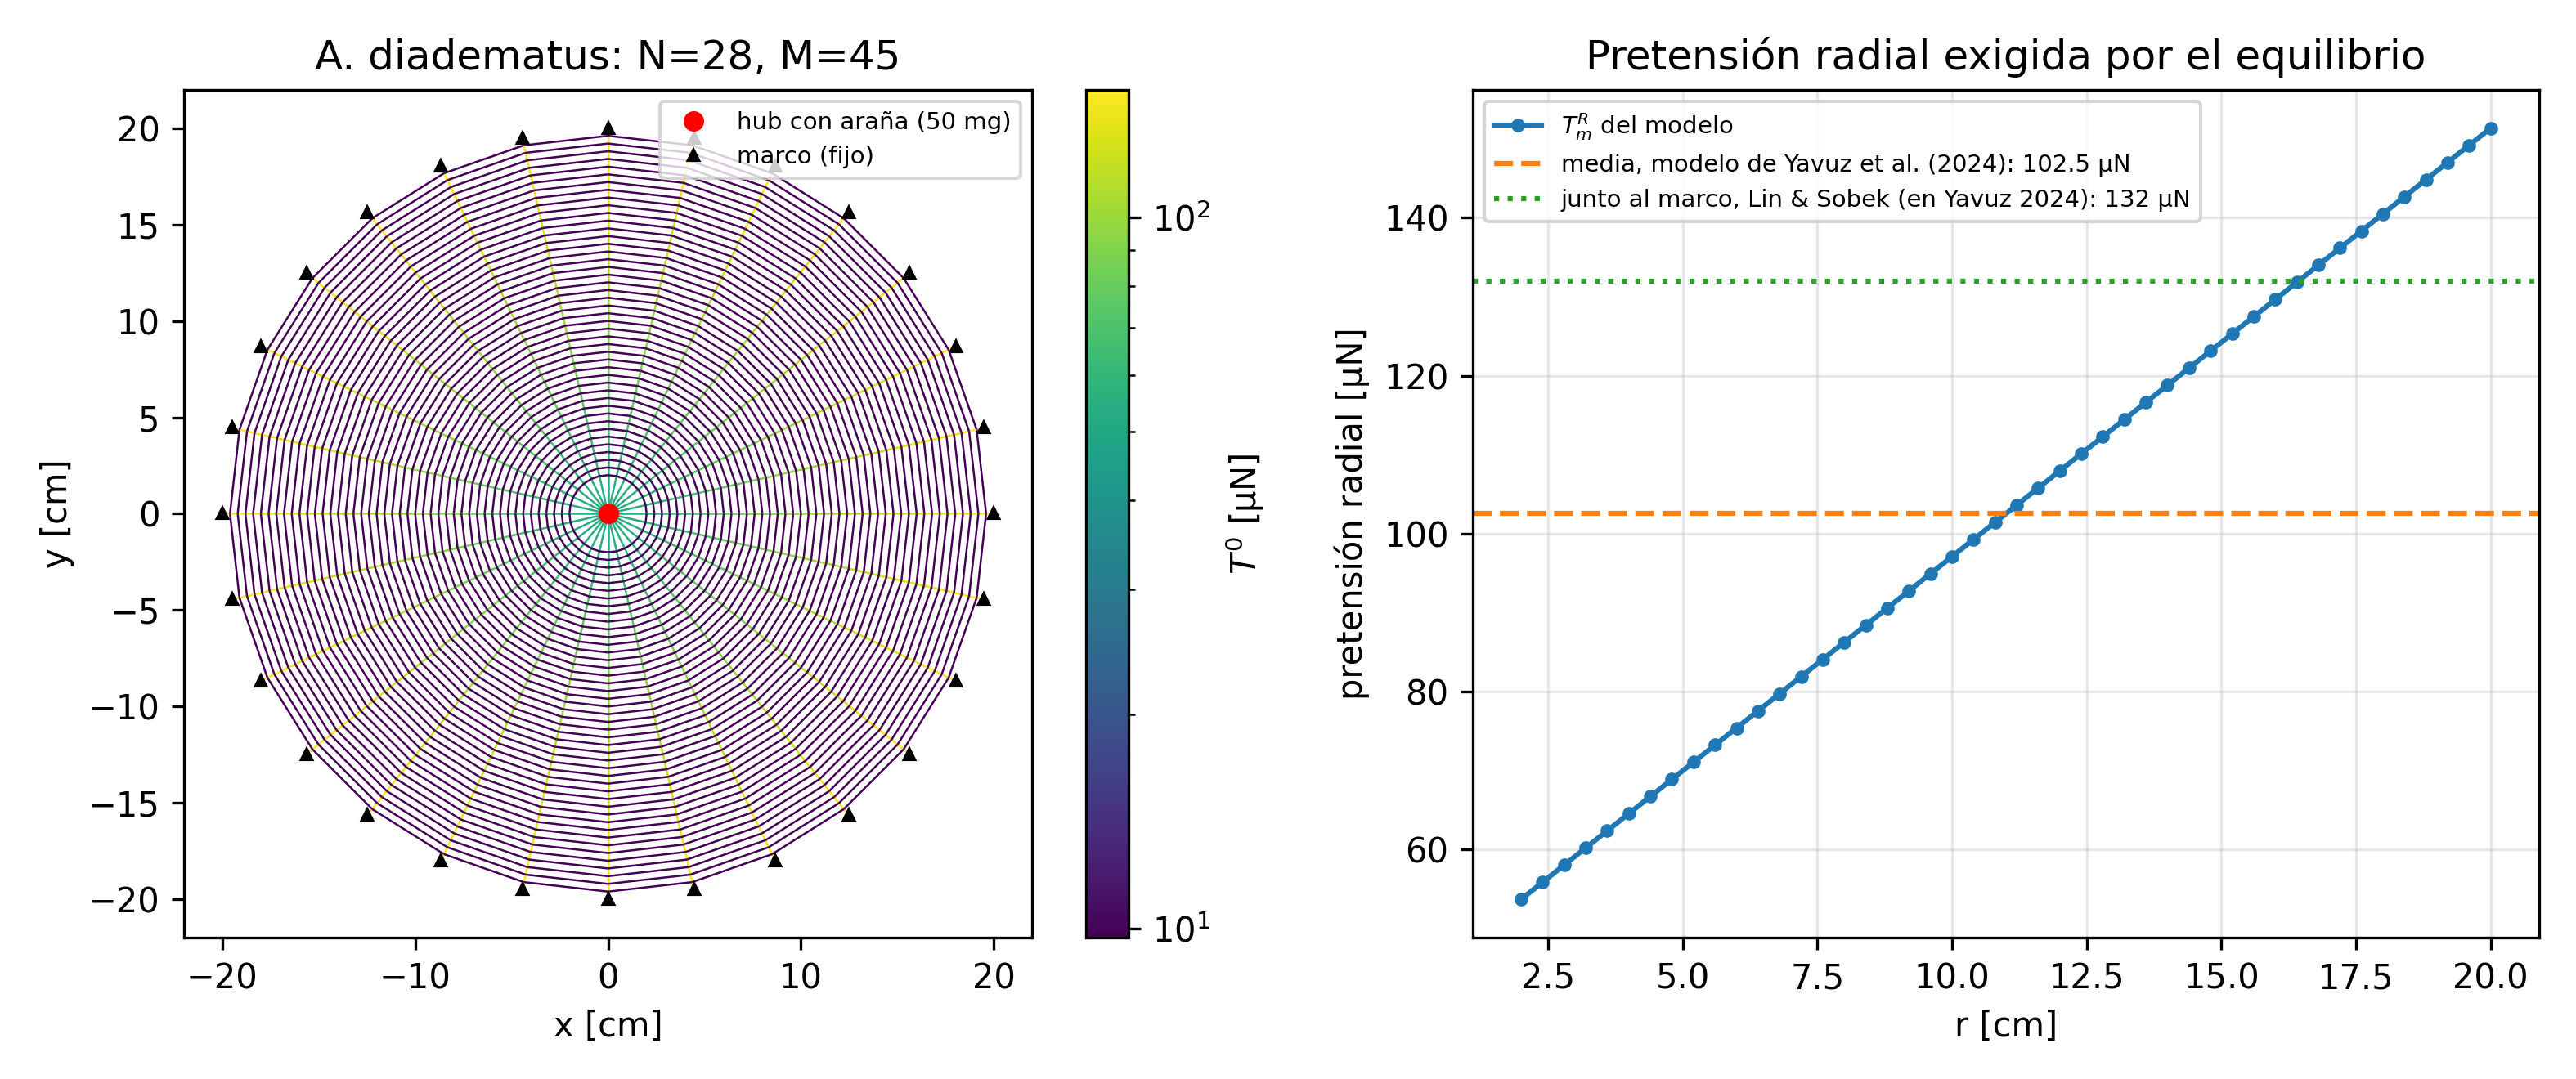
\includegraphics[width=\textwidth]{fig01_geometria.png}
\caption{Configuración base y pretensión radial exigida por el equilibrio
\eqref{eq:recurrencia}, comparada con valores de la literatura.}
\end{figure}

La red tiene 1261 modos transversales, entre 2.50 y 3973 Hz, de los cuales
197 caen en la banda de 1 a 1000 Hz. Tiene además 2522 modos en el plano,
entre 65.6 Hz y 169 kHz. La familia en el plano llega a frecuencias mucho
mayores porque incluye los modos longitudinales, controlados por
$\kappa=EA/L$, que para los radiales es unas mil veces mayor que $T^0/L$.

\begin{figure}[H]
\centering
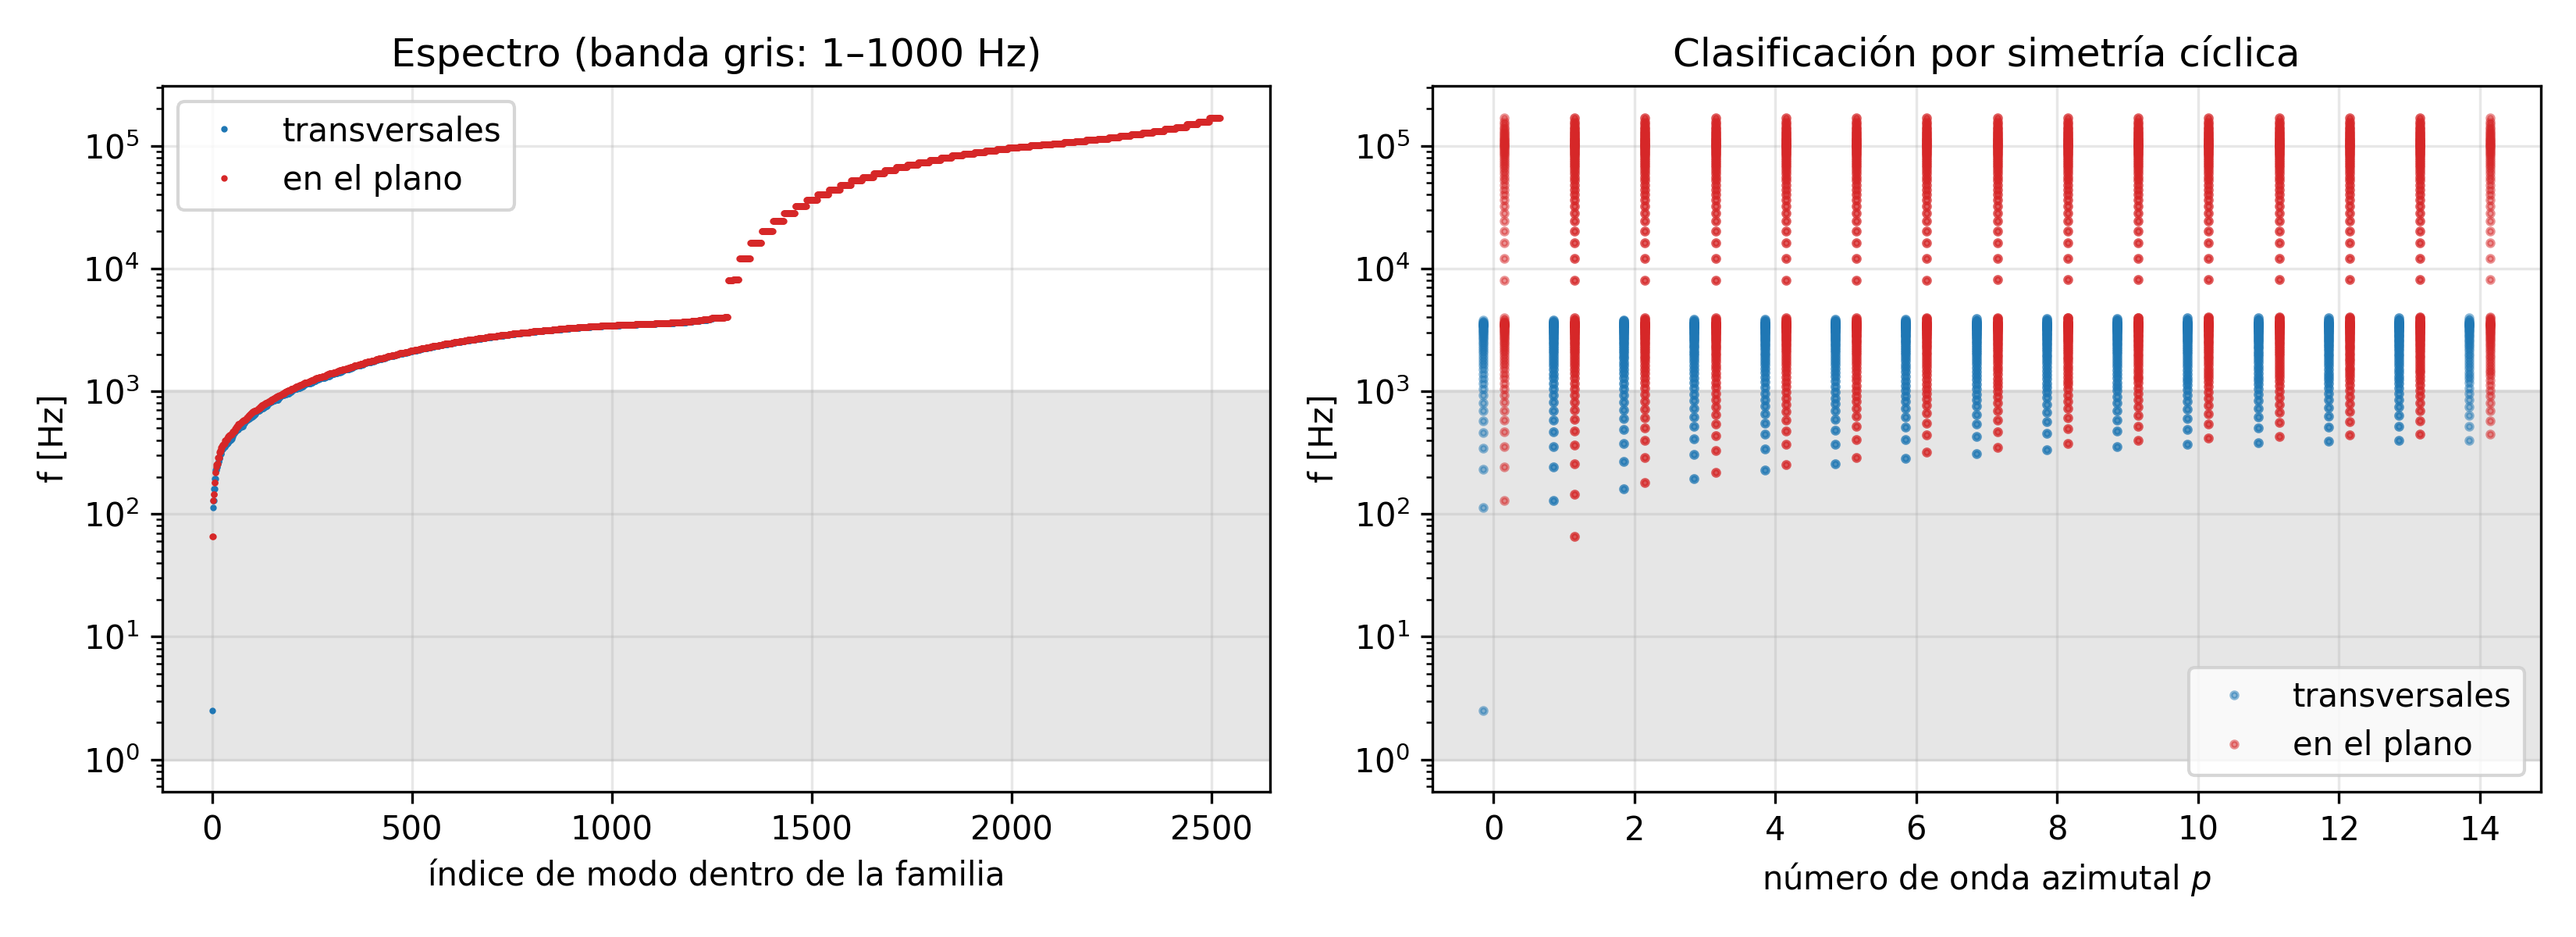
\includegraphics[width=\textwidth]{fig02_espectro.png}
\caption{Izquierda: espectro de frecuencias naturales por familia.
Derecha: clasificación por número de onda azimutal $p$.}
\end{figure}

El primer modo transversal (2.50 Hz) es el rebote de la araña sobre la red:
la masa de 50 mg oscila contra la rigidez transversal de los 28 radiales. El
segundo modo (112.9 Hz, $p=0$) es el fundamental axisimétrico de la red, con
la araña actuando casi como un punto fijo. A partir de él los modos
aparecen en pares degenerados con $p\geq1$, como exige la simetría cíclica
(figura~\ref{fig:modosT}). En el plano, el primer modo (65.6 Hz, $p=1$)
corresponde a la traslación de la araña en el plano de la red.

\begin{figure}[H]
\centering
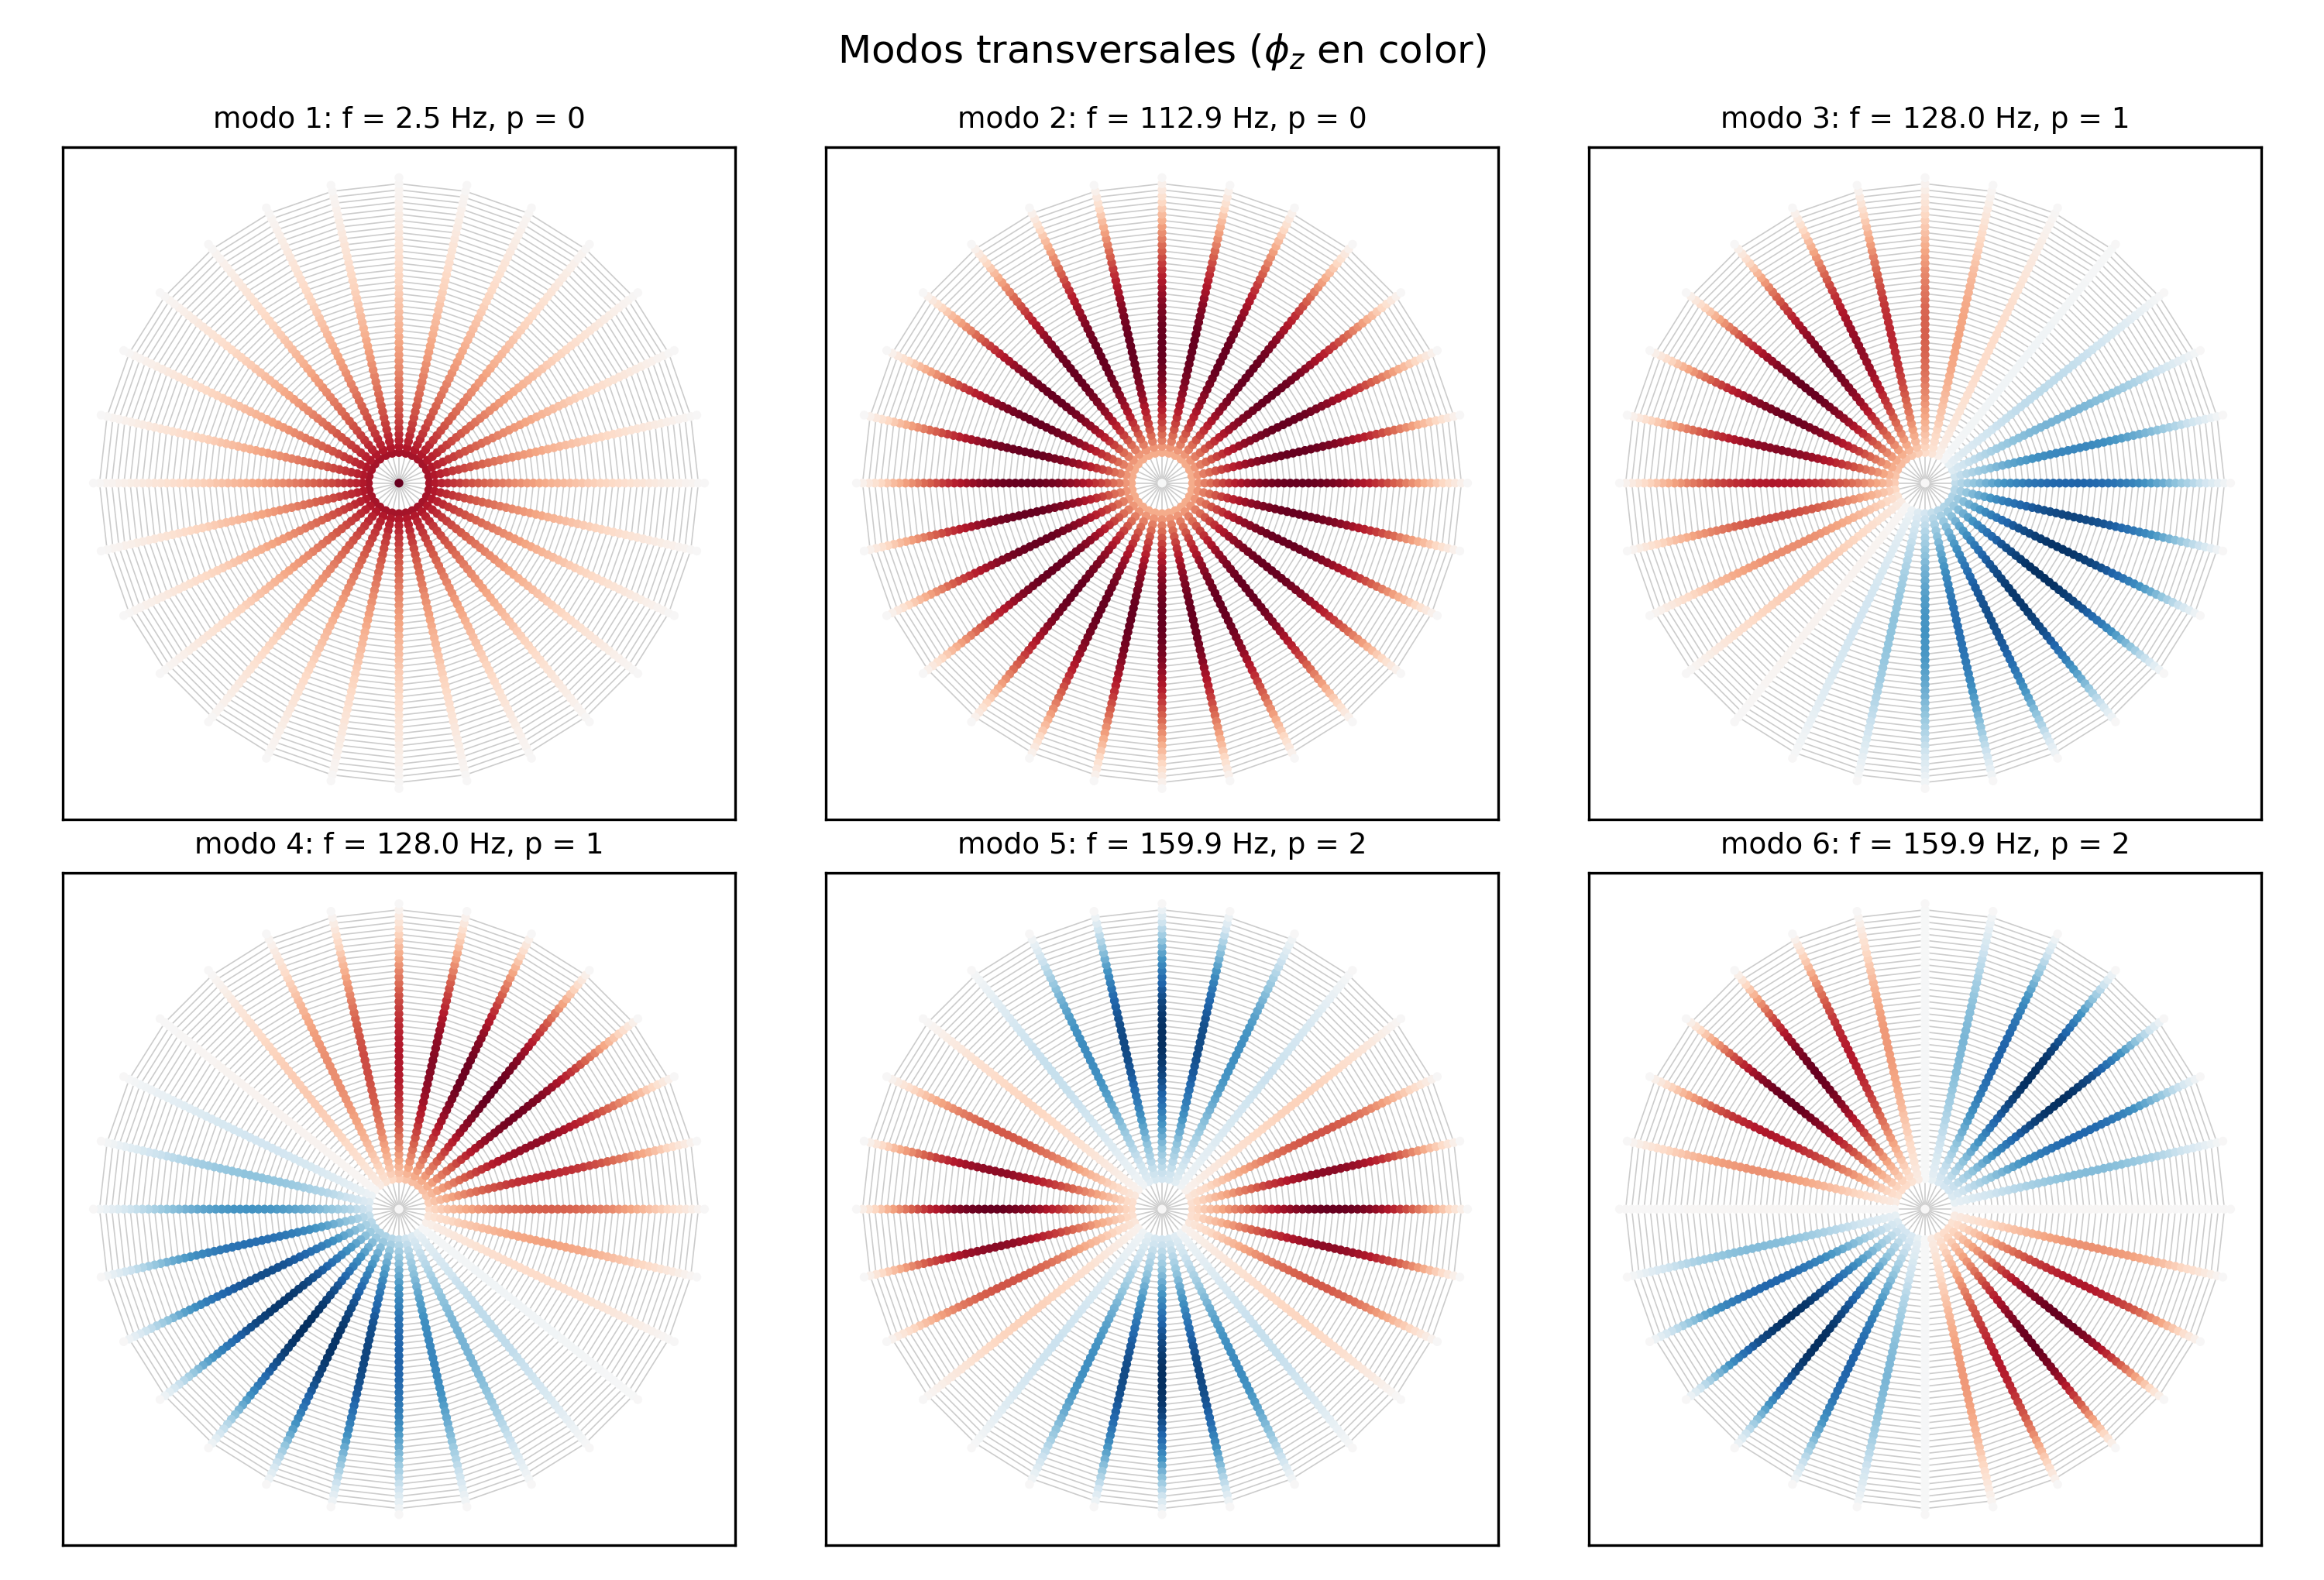
\includegraphics[width=\textwidth]{fig03_modos_transversales.png}
\caption{Primeros seis modos transversales; el color indica $\phi_z$.}
\label{fig:modosT}
\end{figure}

\begin{figure}[H]
\centering
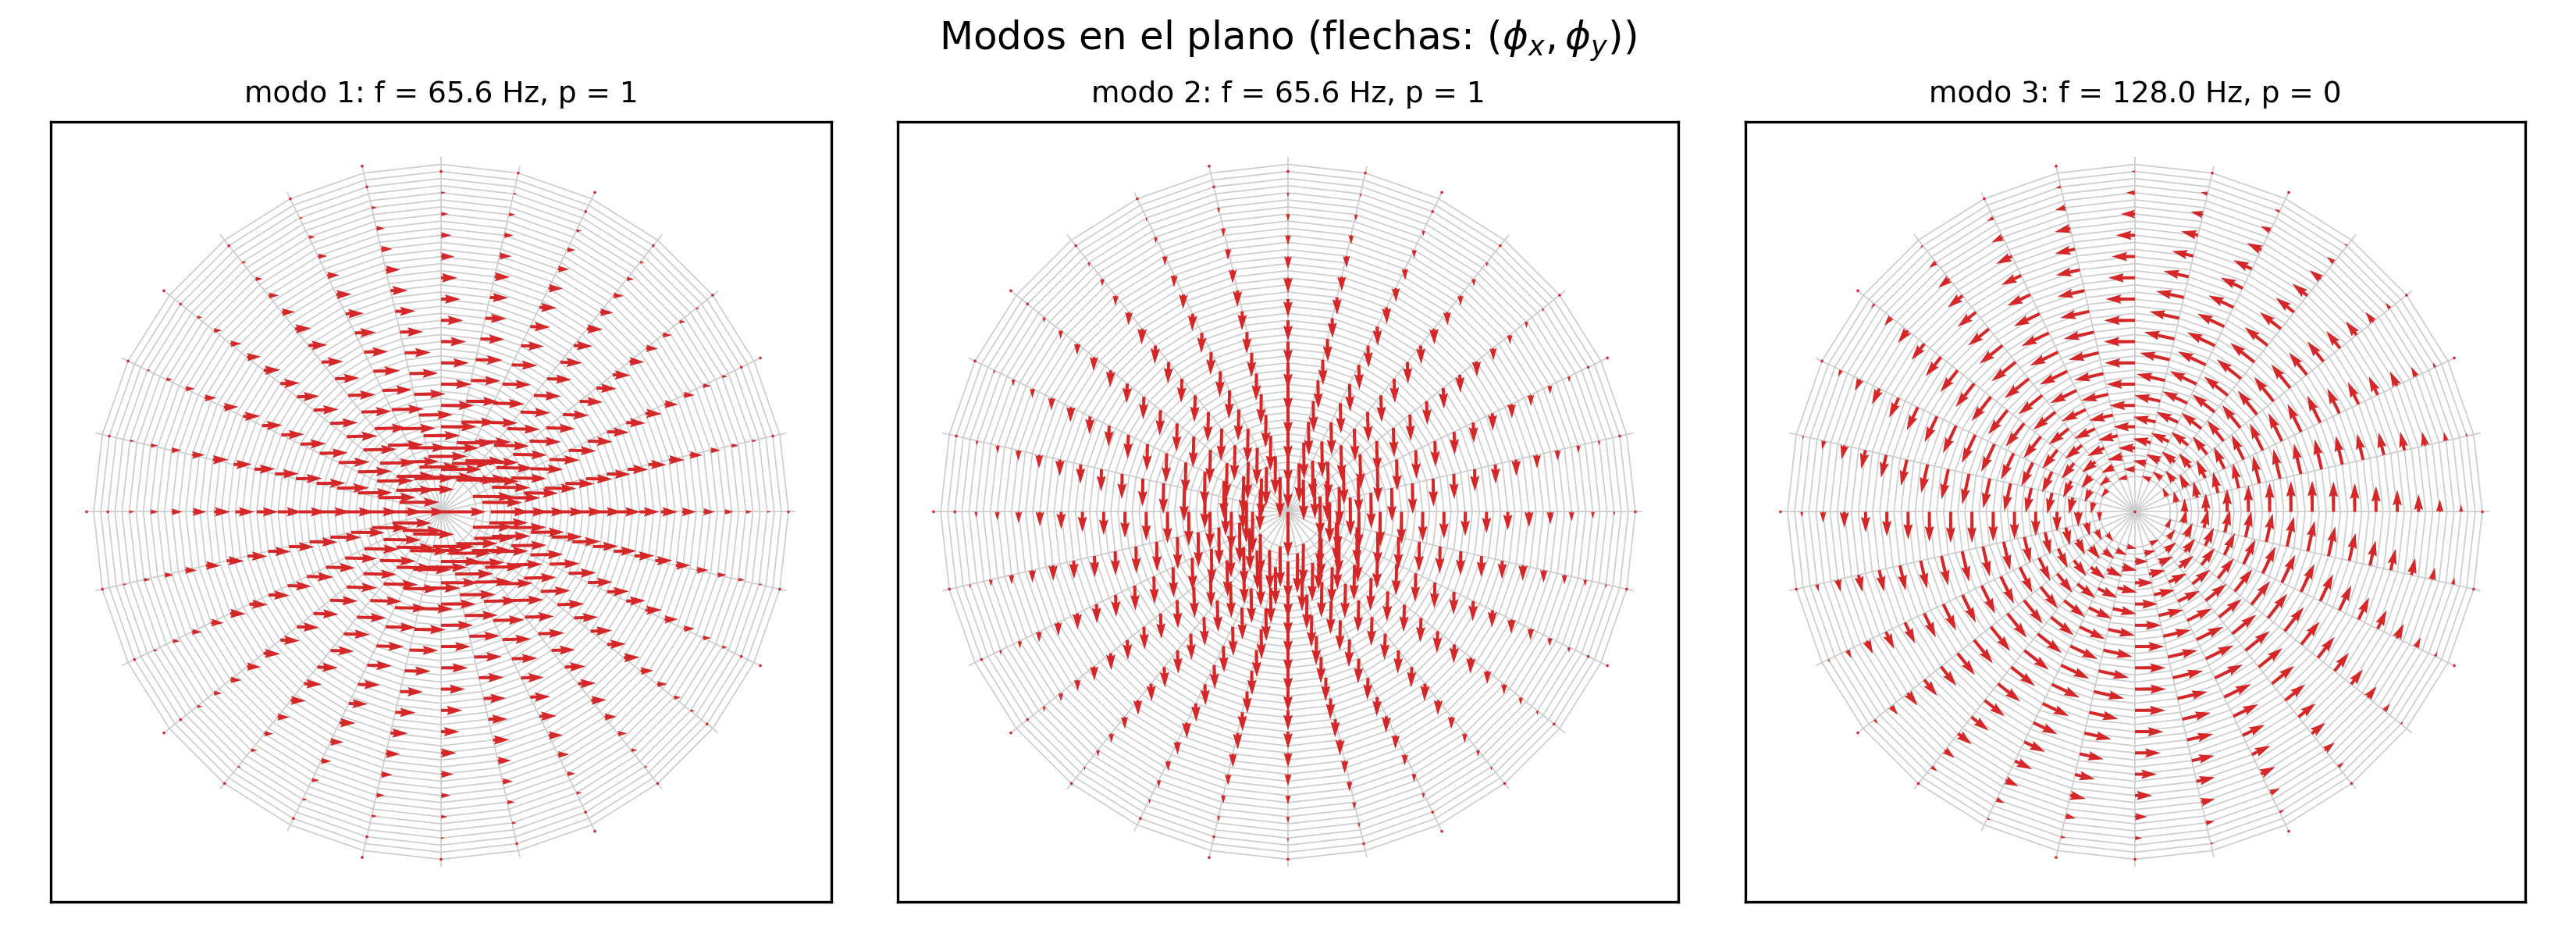
\includegraphics[width=\textwidth]{fig04_modos_plano.png}
\caption{Primeros modos en el plano; las flechas indican $(\phi_x,\phi_y)$.}
\end{figure}

\begin{figure}[H]
\centering
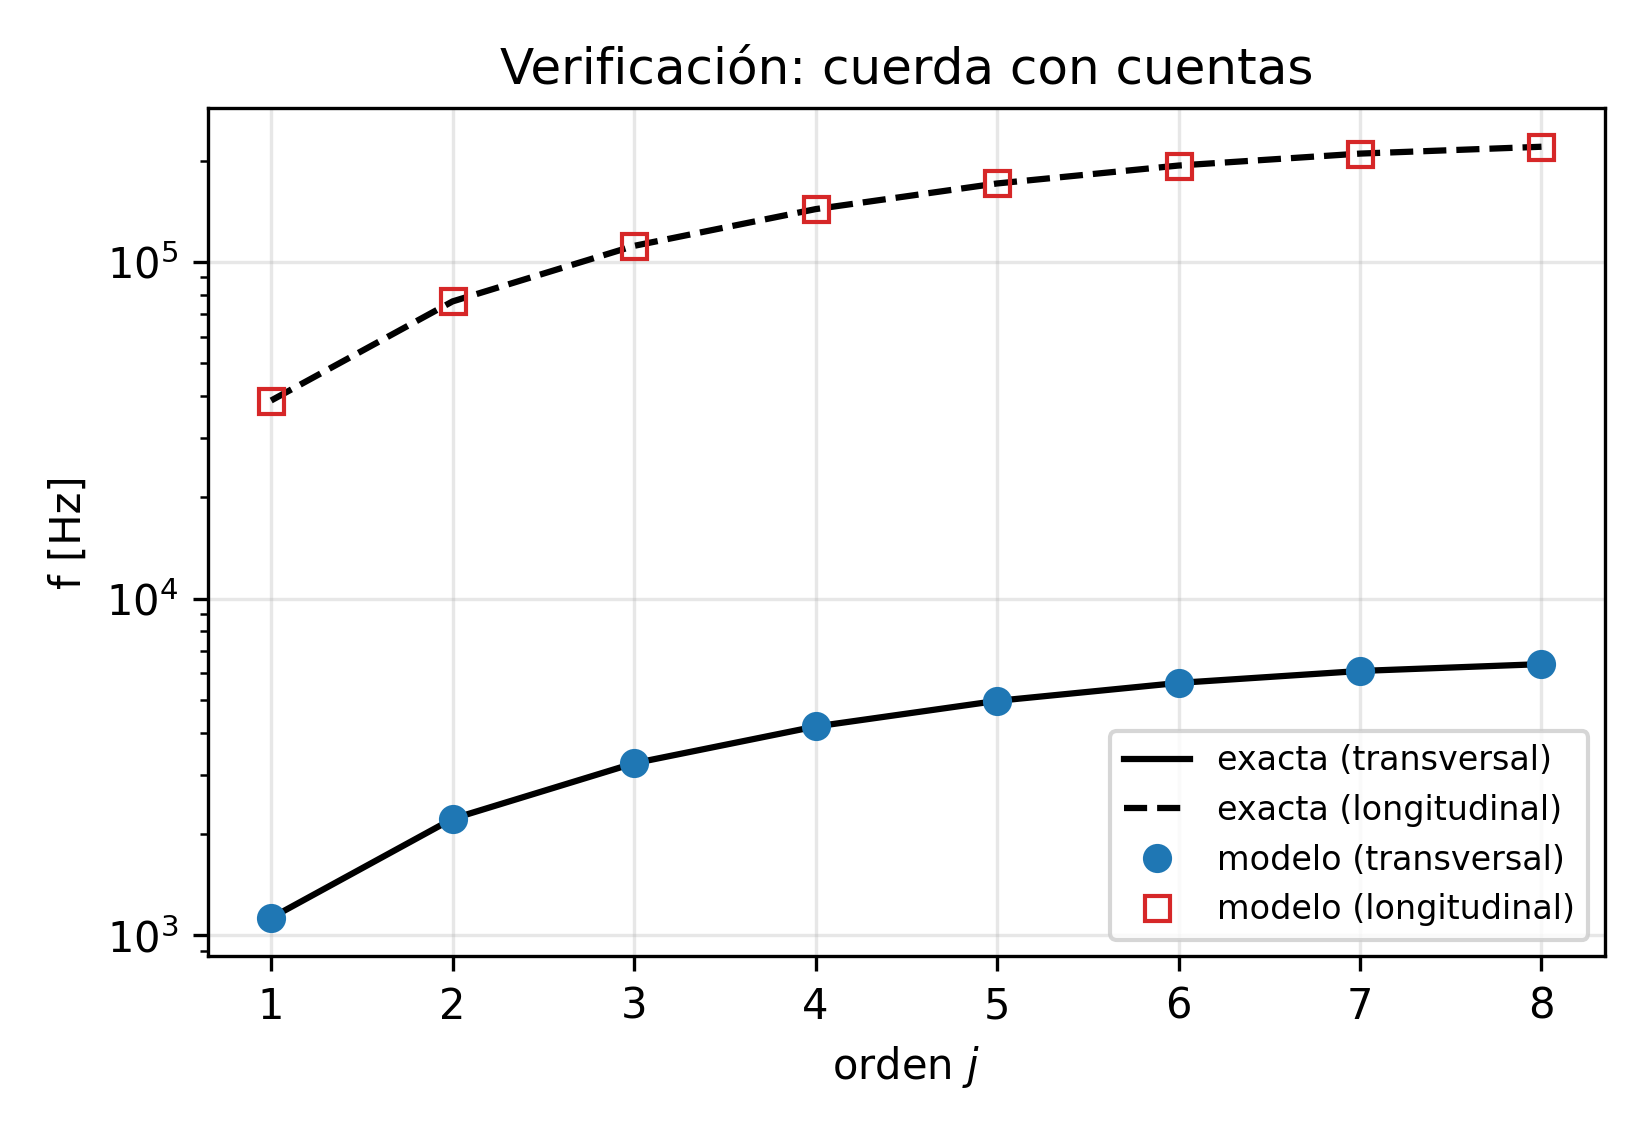
\includegraphics[width=0.55\textwidth]{fig05_benchmark.png}
\caption{Verificación contra la cuerda con cuentas.}
\label{fig:bench}
\end{figure}

\subsection{Respuesta temporal ante una perturbación impulsional}

Se aplicó un impulso transversal en el nodo $(0,16)$, a 8 cm del hub, que
representa una presa atrapada \cite{yavuz2024}. Su magnitud se escaló para
producir un desplazamiento máximo de $\approx0.18$ mm, comparable al
estímulo de 0.21 mm usado por Mortimer et al.\ \cite{mortimer2018}. Se
observó la respuesta en nodos del anillo 1, donde se apoyan las patas de la
araña, y en el hub.

\begin{figure}[H]
\centering
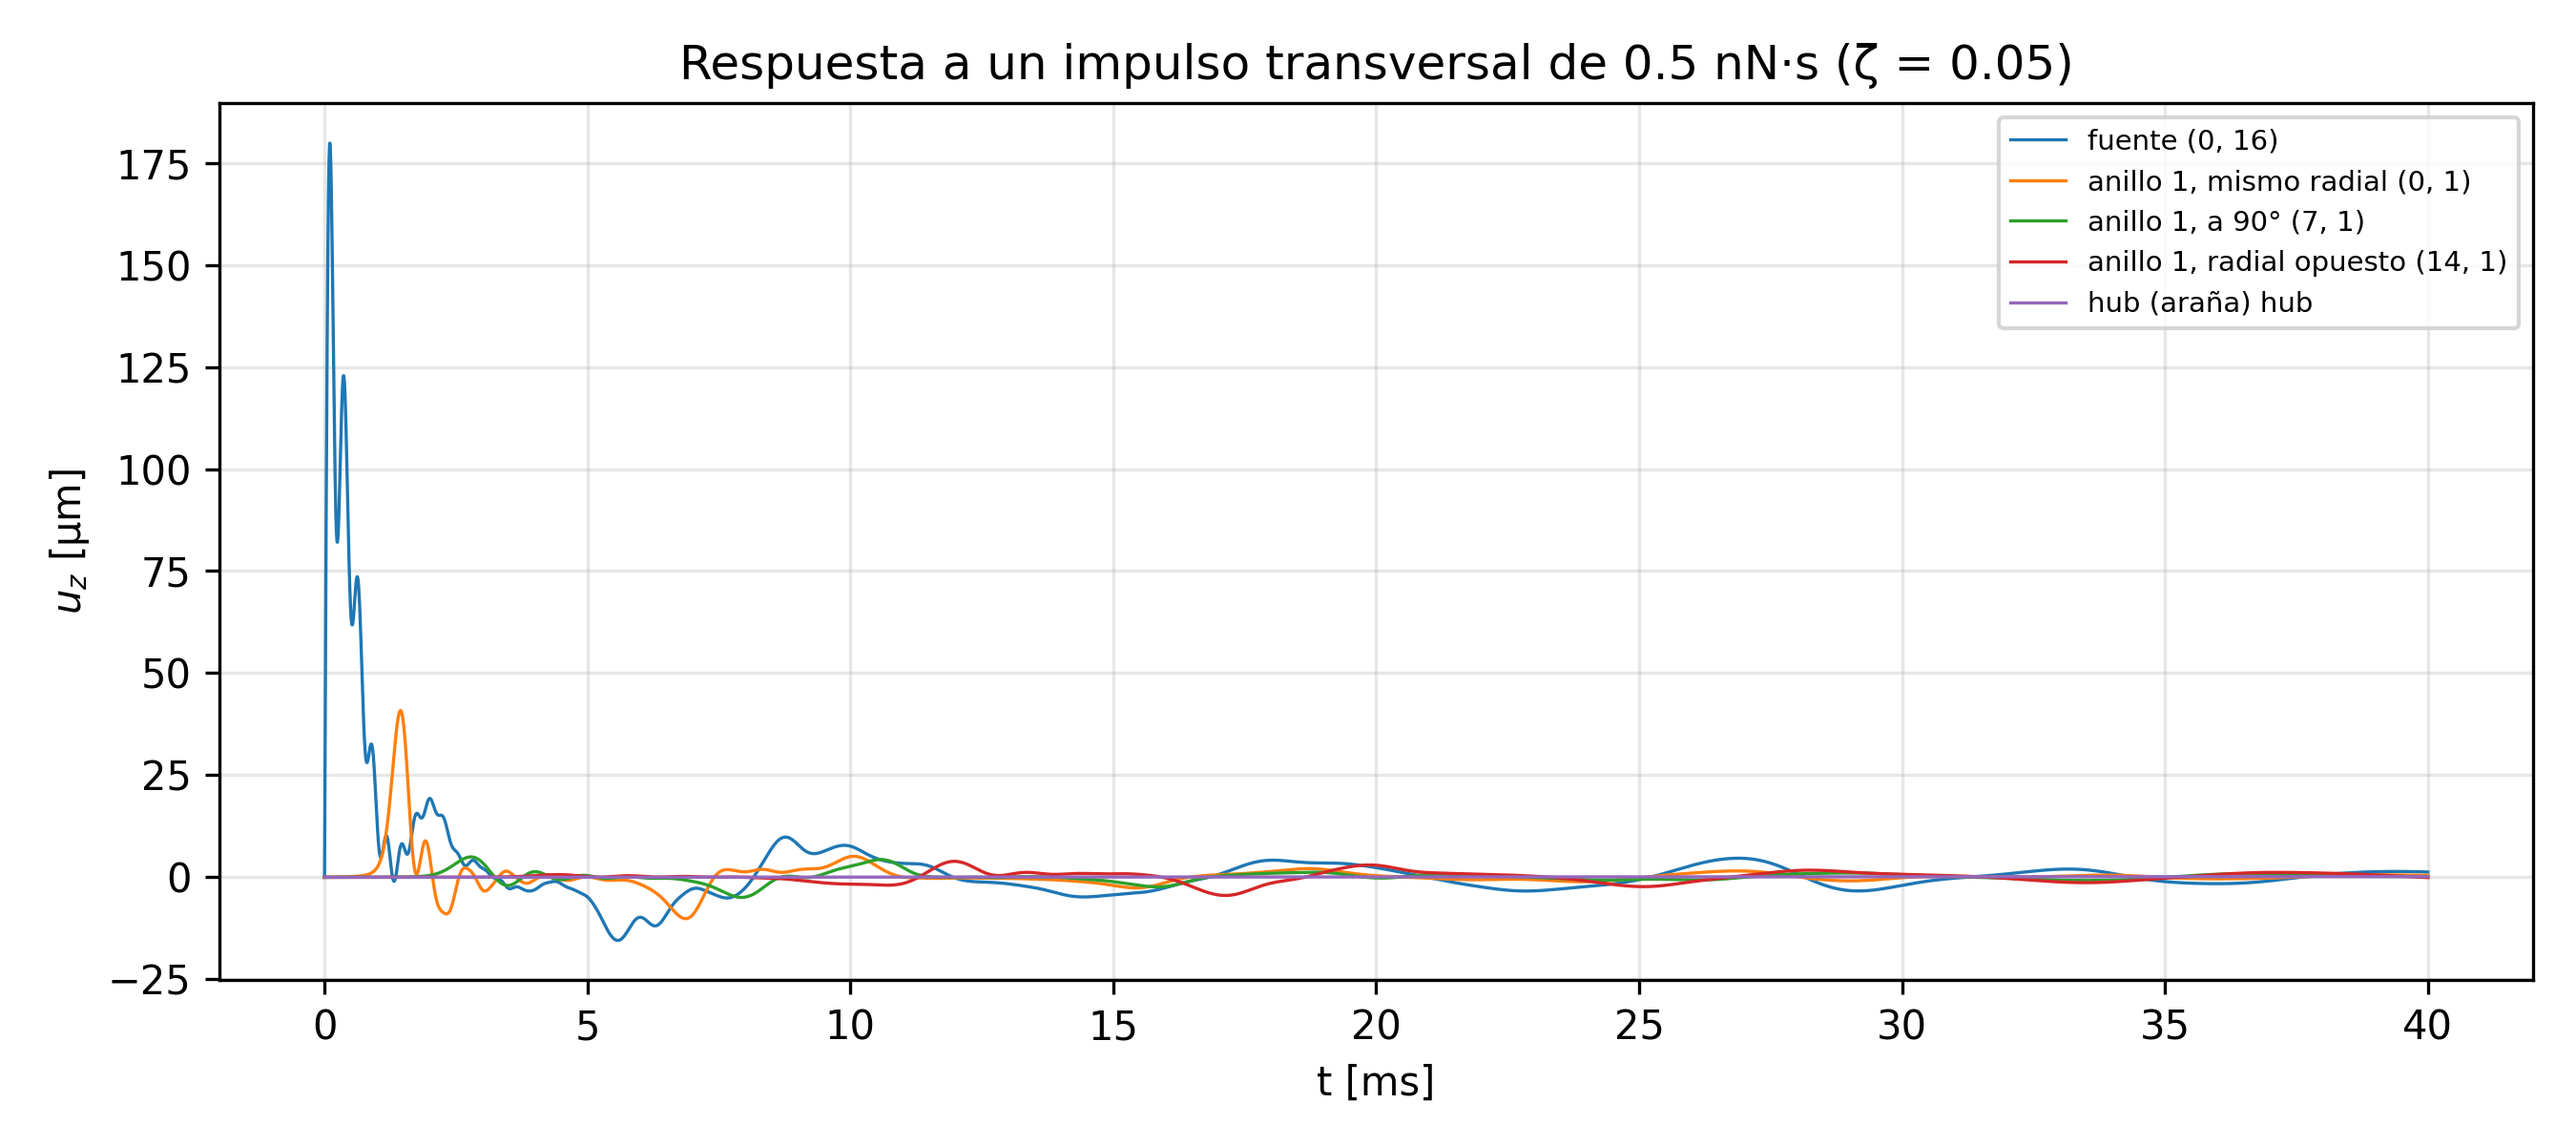
\includegraphics[width=0.9\textwidth]{fig06_respuesta_impulsional.png}
\caption{Respuesta impulsional $u_z(t)$ en la fuente, en tres observadores
del anillo 1 y en el hub.}
\end{figure}

\begin{figure}[H]
\centering
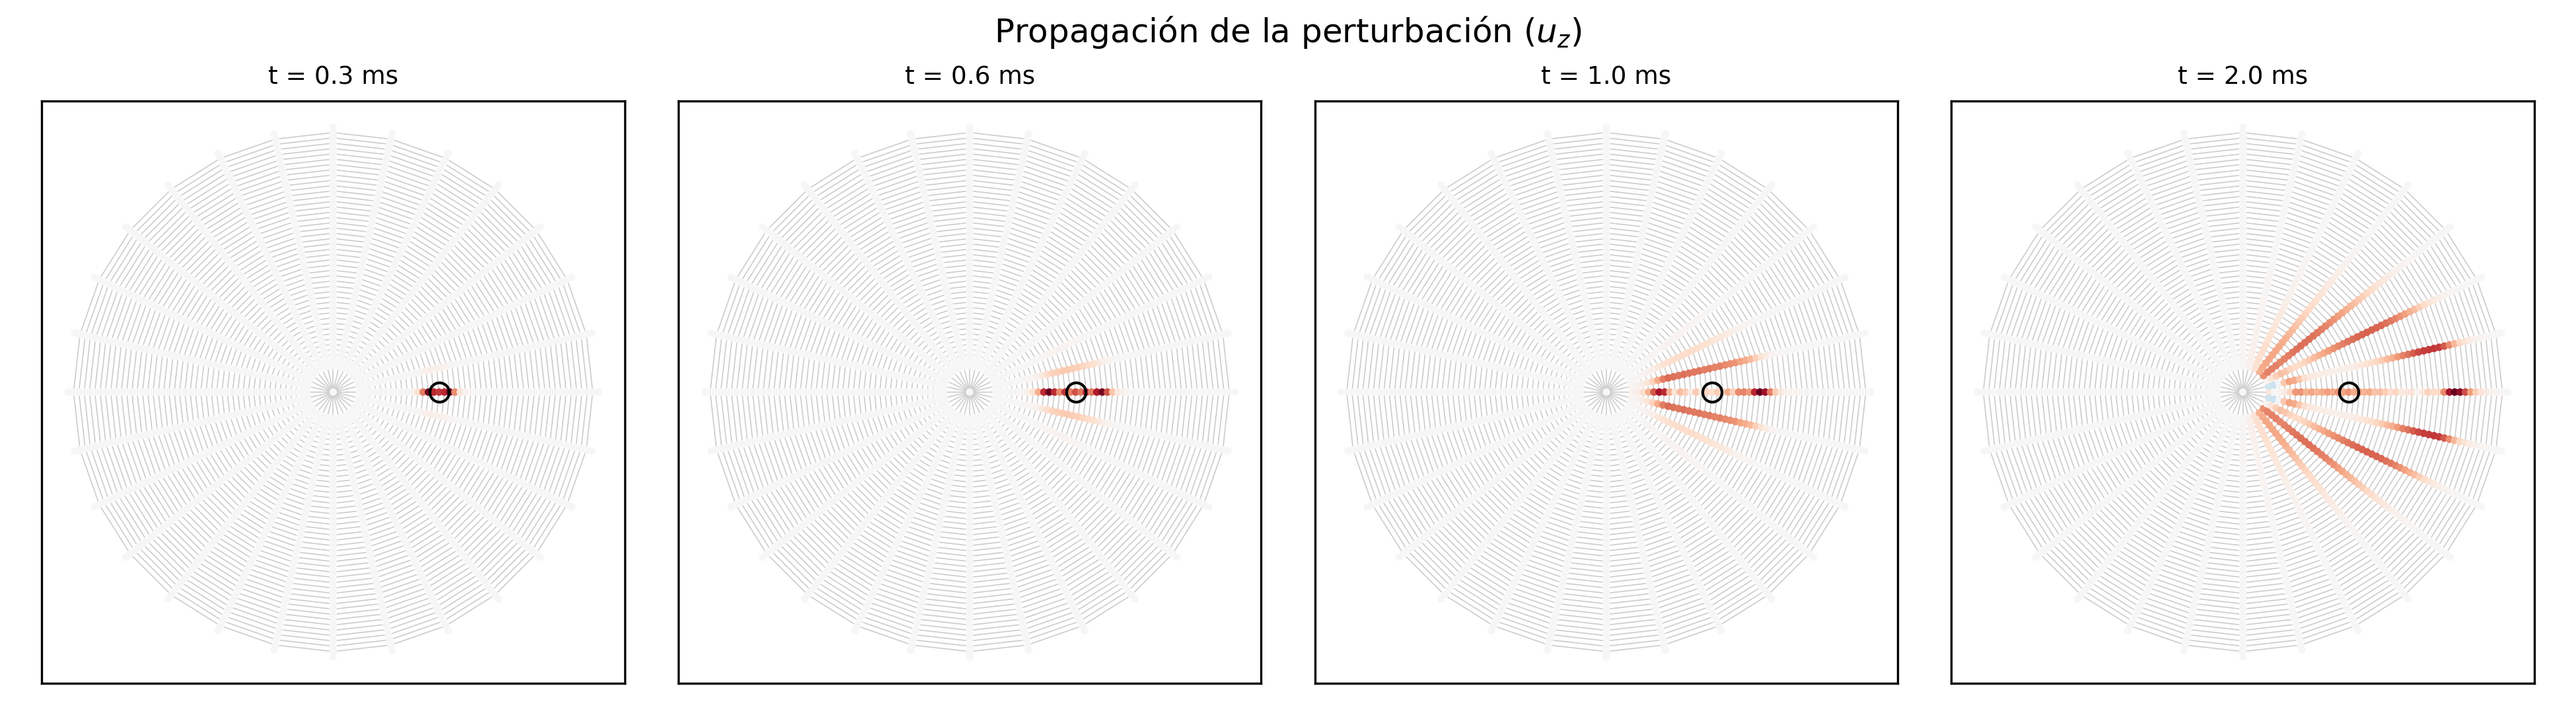
\includegraphics[width=\textwidth]{fig07_instantaneas.png}
\caption{Propagación de la perturbación. El frente viaja principalmente por
el radial de la fuente y se reparte hacia los radiales vecinos a través de
la espiral.}
\end{figure}

La velocidad aparente de la onda transversal hacia el hub es de 53 m/s.
Este valor es consistente con la estimación $\sqrt{T^R/\lambda_{\text{ef}}}
\approx 47$ m/s, donde $\lambda_{\text{ef}}$ incluye la masa de la espiral
repartida sobre el radial.

\begin{figure}[H]
\centering
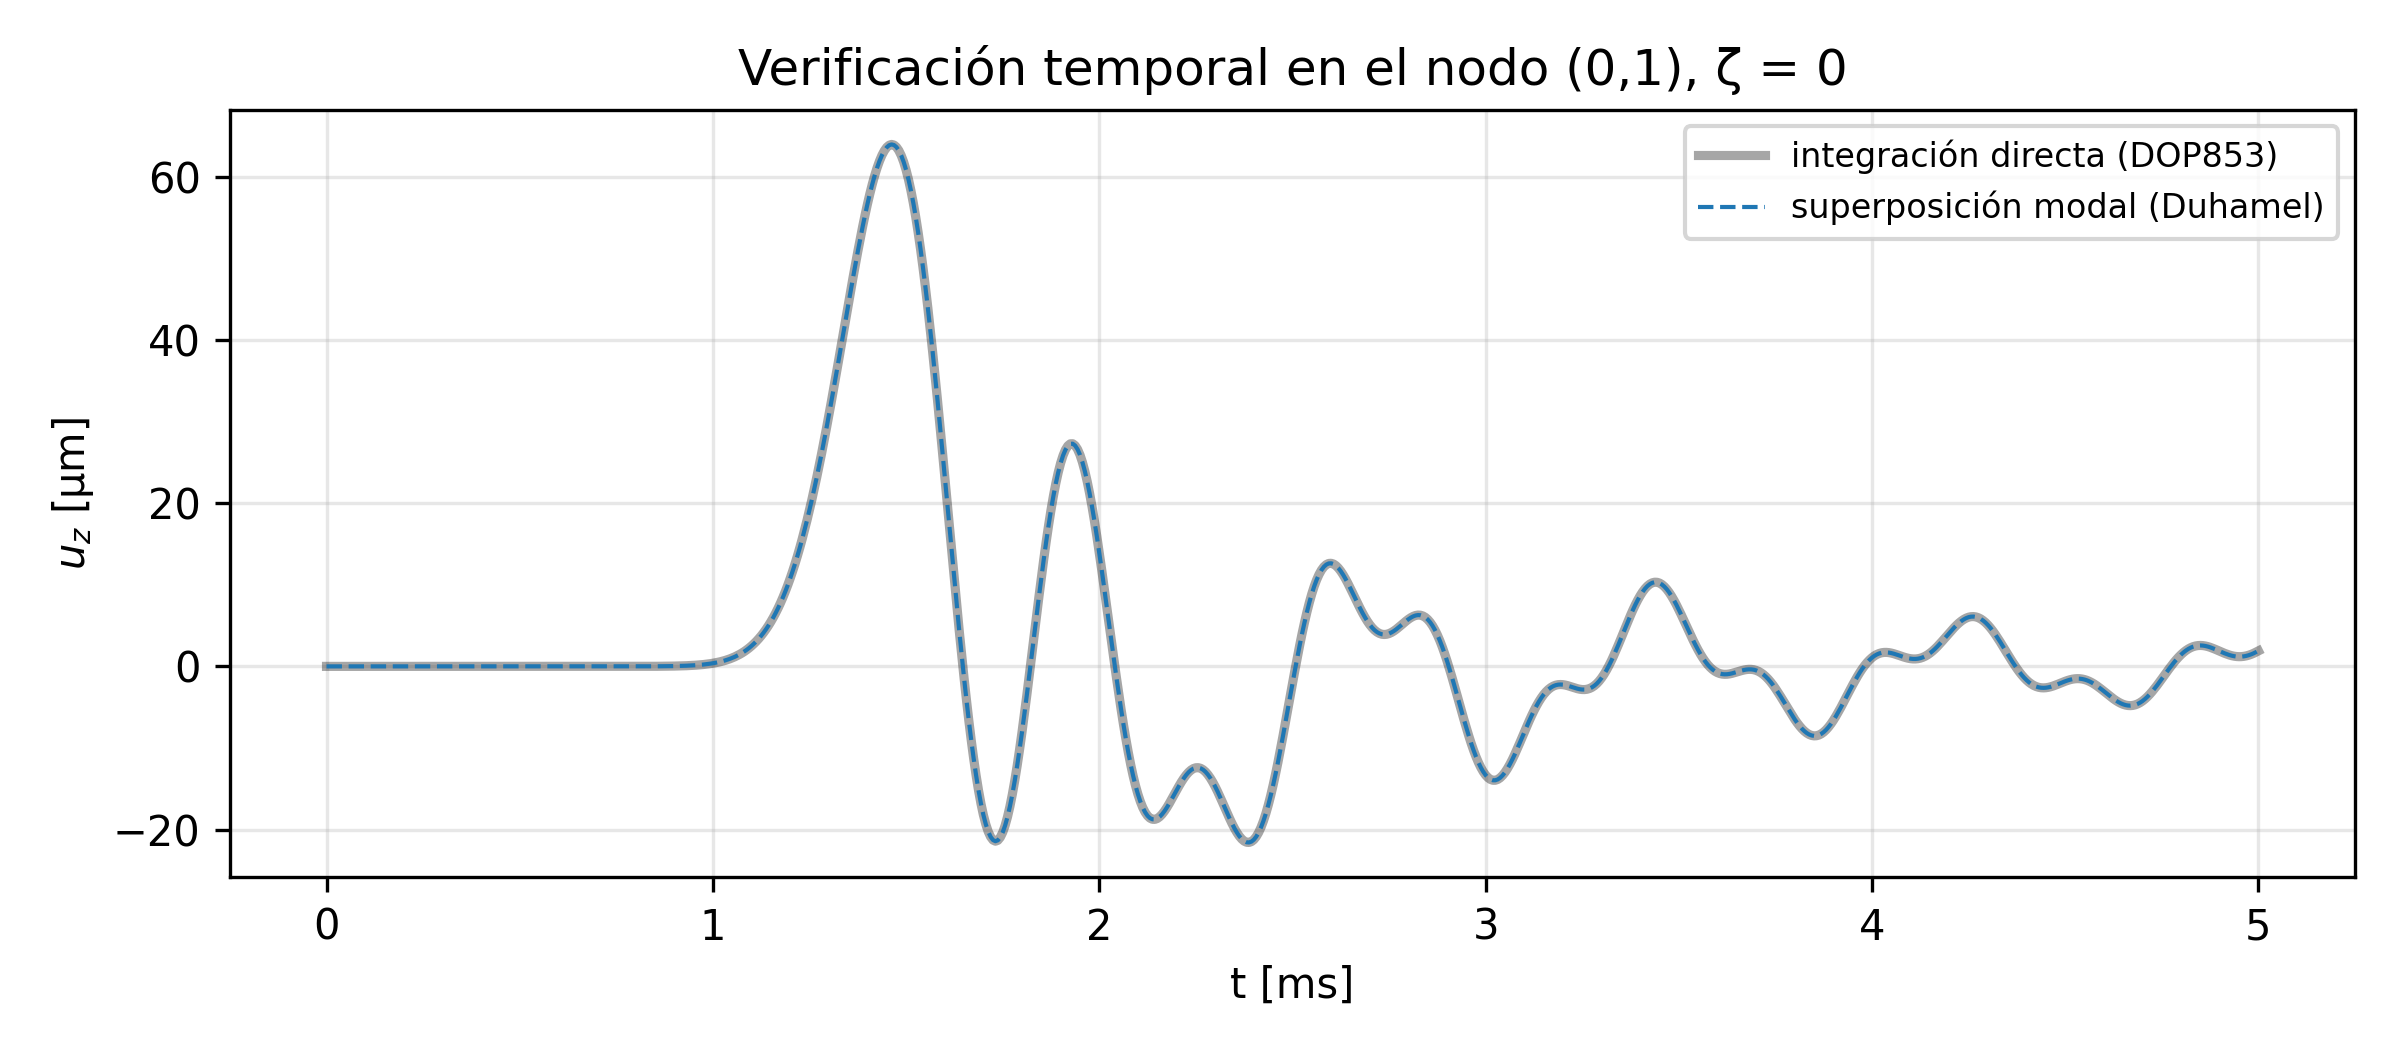
\includegraphics[width=0.85\textwidth]{fig08_verificacion_temporal.png}
\caption{Verificación de la superposición modal contra la integración
numérica directa del subsistema transversal.}
\end{figure}

\subsection{Función de transferencia e índice de transmisión}

\begin{figure}[H]
\centering
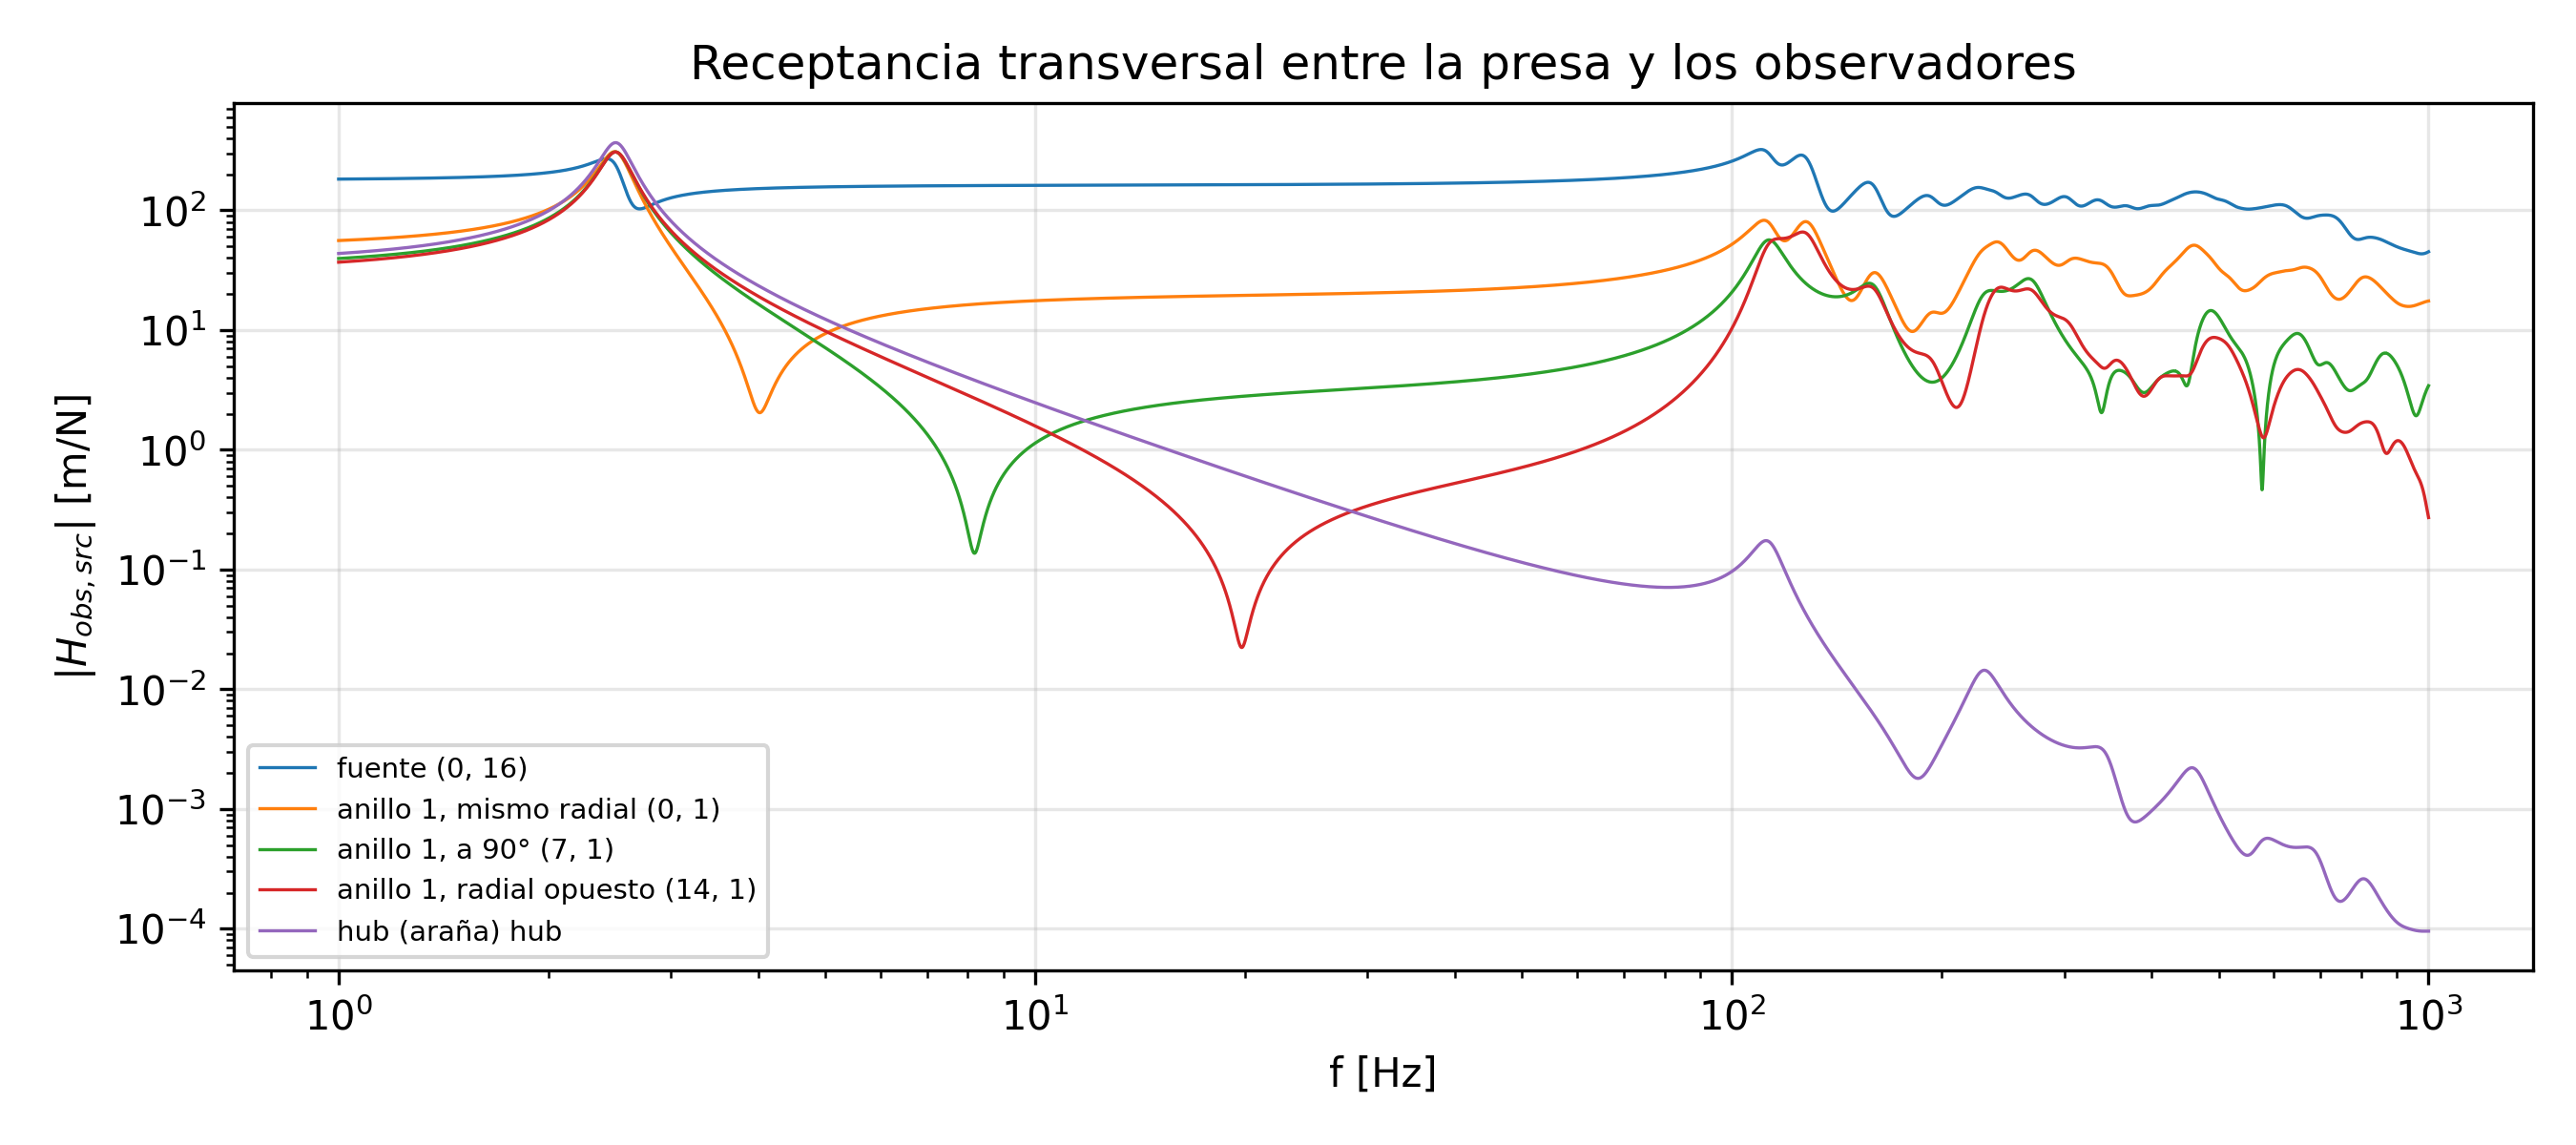
\includegraphics[width=0.9\textwidth]{fig09_transferencia.png}
\caption{Módulo de la receptancia $|H_{obs,src}(\omega)|$ entre la presa y
los observadores.}
\label{fig:H}
\end{figure}

En la figura~\ref{fig:H} se distinguen tres regiones. Cerca de 2.5 Hz,
todos los nodos se mueven juntos con la araña (modo de rebote), por lo que
la respuesta no contiene información direccional. Entre unos 3 y 100 Hz,
que incluye la banda de vibración de presas atrapadas (5--30 Hz
\cite{landolfa1996}), cada observador tiene una antirresonancia a una
frecuencia distinta y las amplitudes difieren en uno a dos órdenes de
magnitud. Por encima de 100 Hz aparecen las resonancias propias de la red.

\begin{figure}[H]
\centering
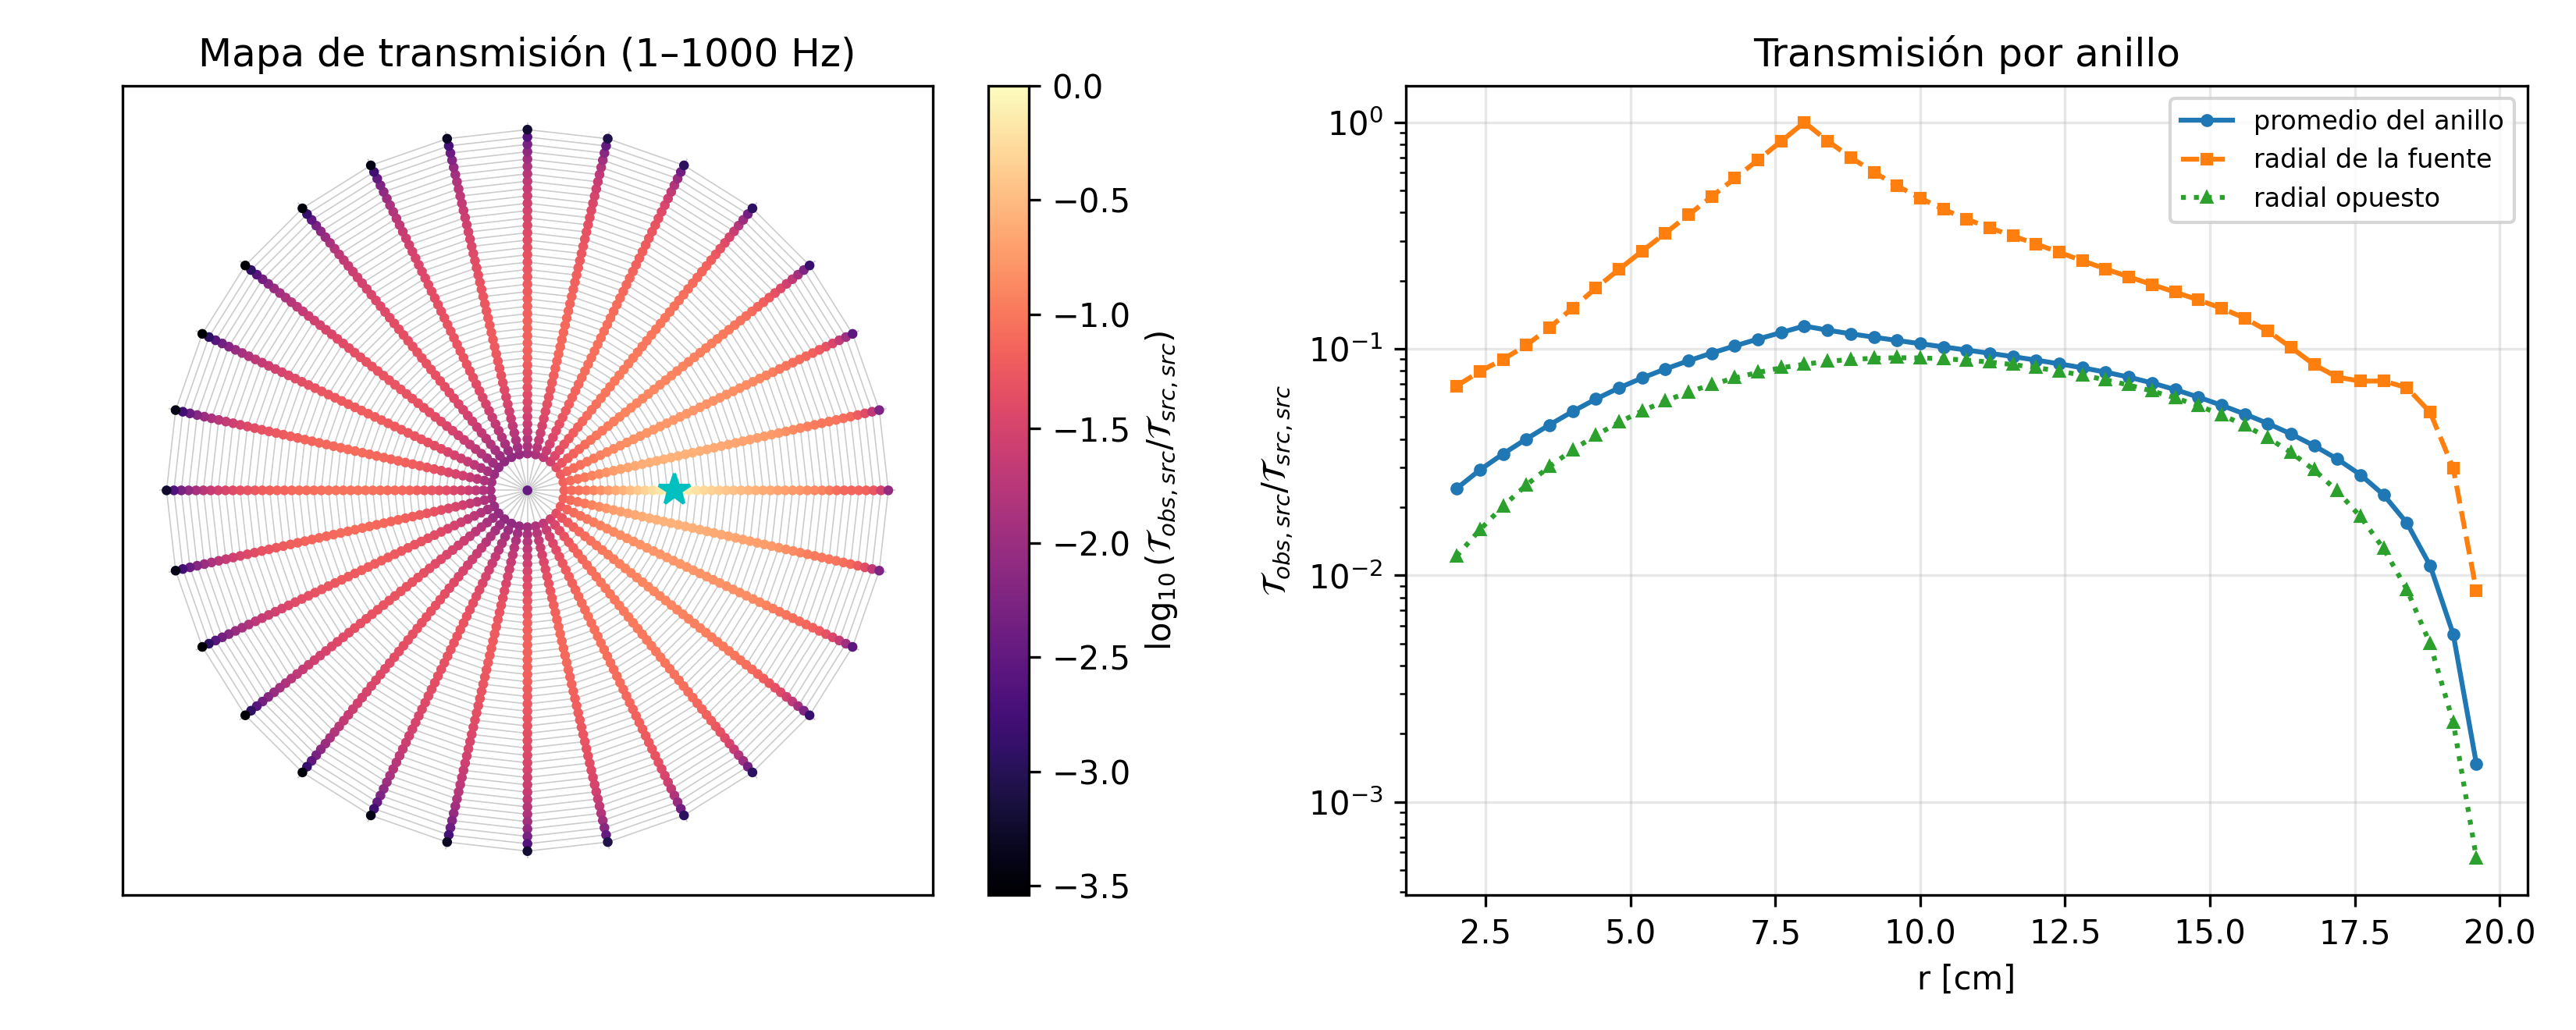
\includegraphics[width=\textwidth]{fig10_mapa_transmision.png}
\caption{Índice de transmisión normalizado
$\mathcal{T}_{obs,src}/\mathcal{T}_{src,src}$ en la banda de 1 a 1000 Hz,
para todos los nodos (izquierda) y por anillo (derecha).}
\end{figure}

\begin{figure}[H]
\centering
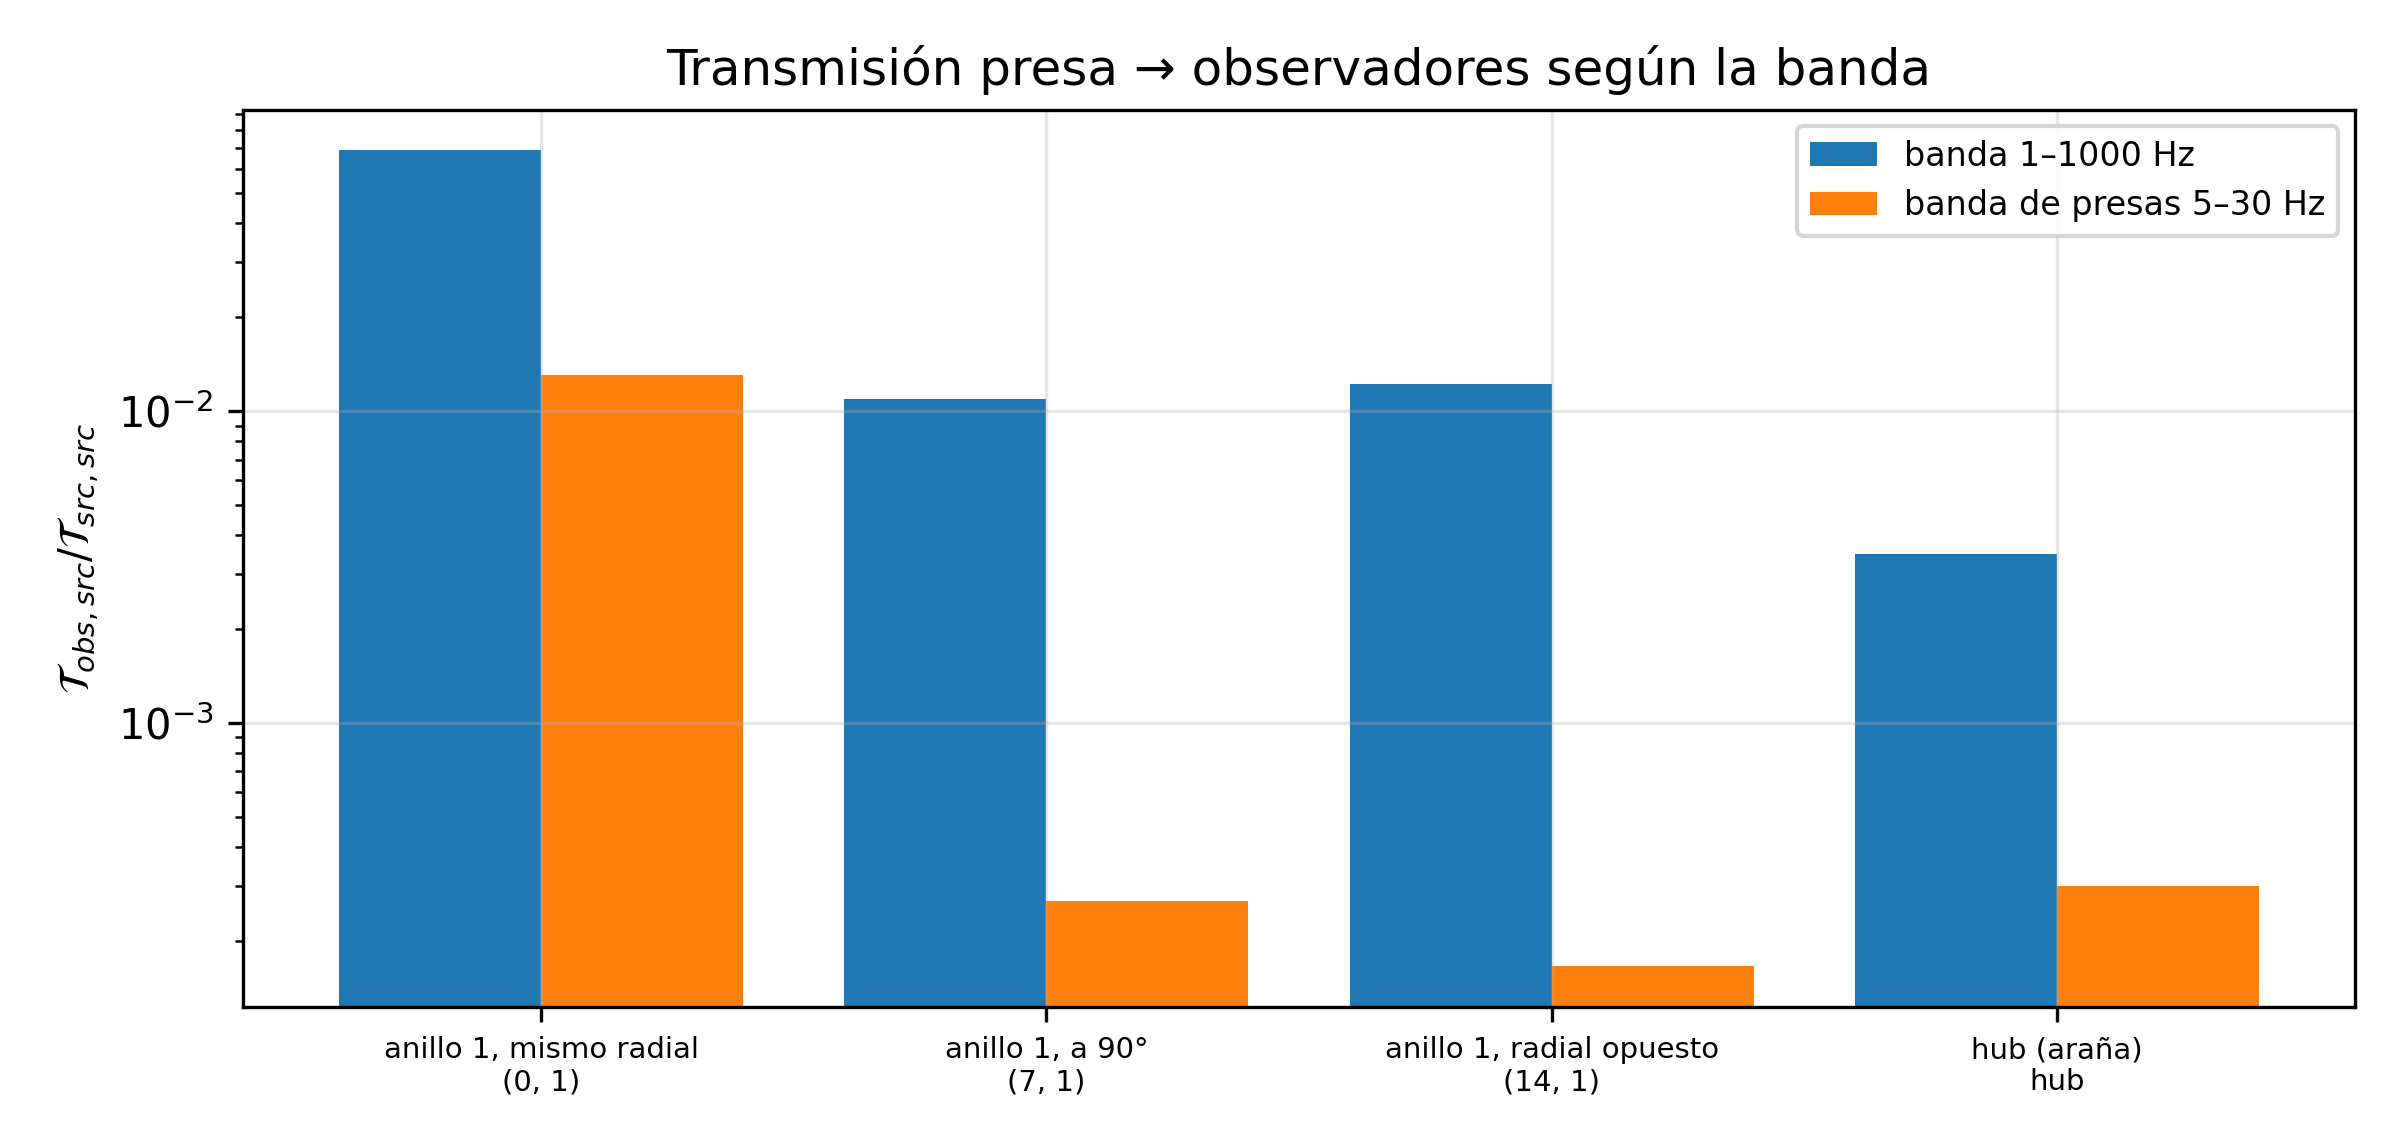
\includegraphics[width=0.8\textwidth]{fig12_transmision_bandas.png}
\caption{Índice normalizado para los observadores en dos bandas.}
\label{fig:bandas}
\end{figure}

\begin{table}[H]
\centering\small
\caption{Índice de transmisión normalizado $\mathcal{T}_{obs,src}/\mathcal{T}_{src,src}$
desde la presa (nodo $(0,16)$).}
\label{tab:T}
\begin{tabular}{@{}lcc@{}}
\toprule
Observador & 1--1000 Hz & 5--30 Hz \\
\midrule
Anillo 1, mismo radial $(0,1)$ & $6.86\times10^{-2}$ & $1.31\times10^{-2}$ \\
Anillo 1, a $90^\circ$ $(7,1)$ & $1.09\times10^{-2}$ & $2.69\times10^{-4}$ \\
Anillo 1, radial opuesto $(14,1)$ & $1.22\times10^{-2}$ & $1.66\times10^{-4}$ \\
Hub (araña) & $3.49\times10^{-3}$ & $3.01\times10^{-4}$ \\
\bottomrule
\end{tabular}
\end{table}

En la banda de 1 a 1000 Hz, el contraste entre el radial de la presa y los
demás es de apenas un factor $\sim6$, porque el índice está dominado por el
modo de rebote y por los modos globales de la red. En la banda de presas, en
cambio, el contraste sube a un factor 50--80 ($\approx17$--19 dB), lo que
indica que la información direccional está concentrada en esa banda. A lo
largo del radial de la presa, la amplitud cae $\approx19$ dB en 6 cm en esa
banda, del mismo orden que la atenuación transversal de 22 dB en unos 12 cm
medida por Landolfa y Barth en \textit{Nephila clavipes}
\cite{landolfa1996}. La comparación es solo orientativa, porque se trata de
otra especie y de otra métrica.

\begin{figure}[H]
\centering
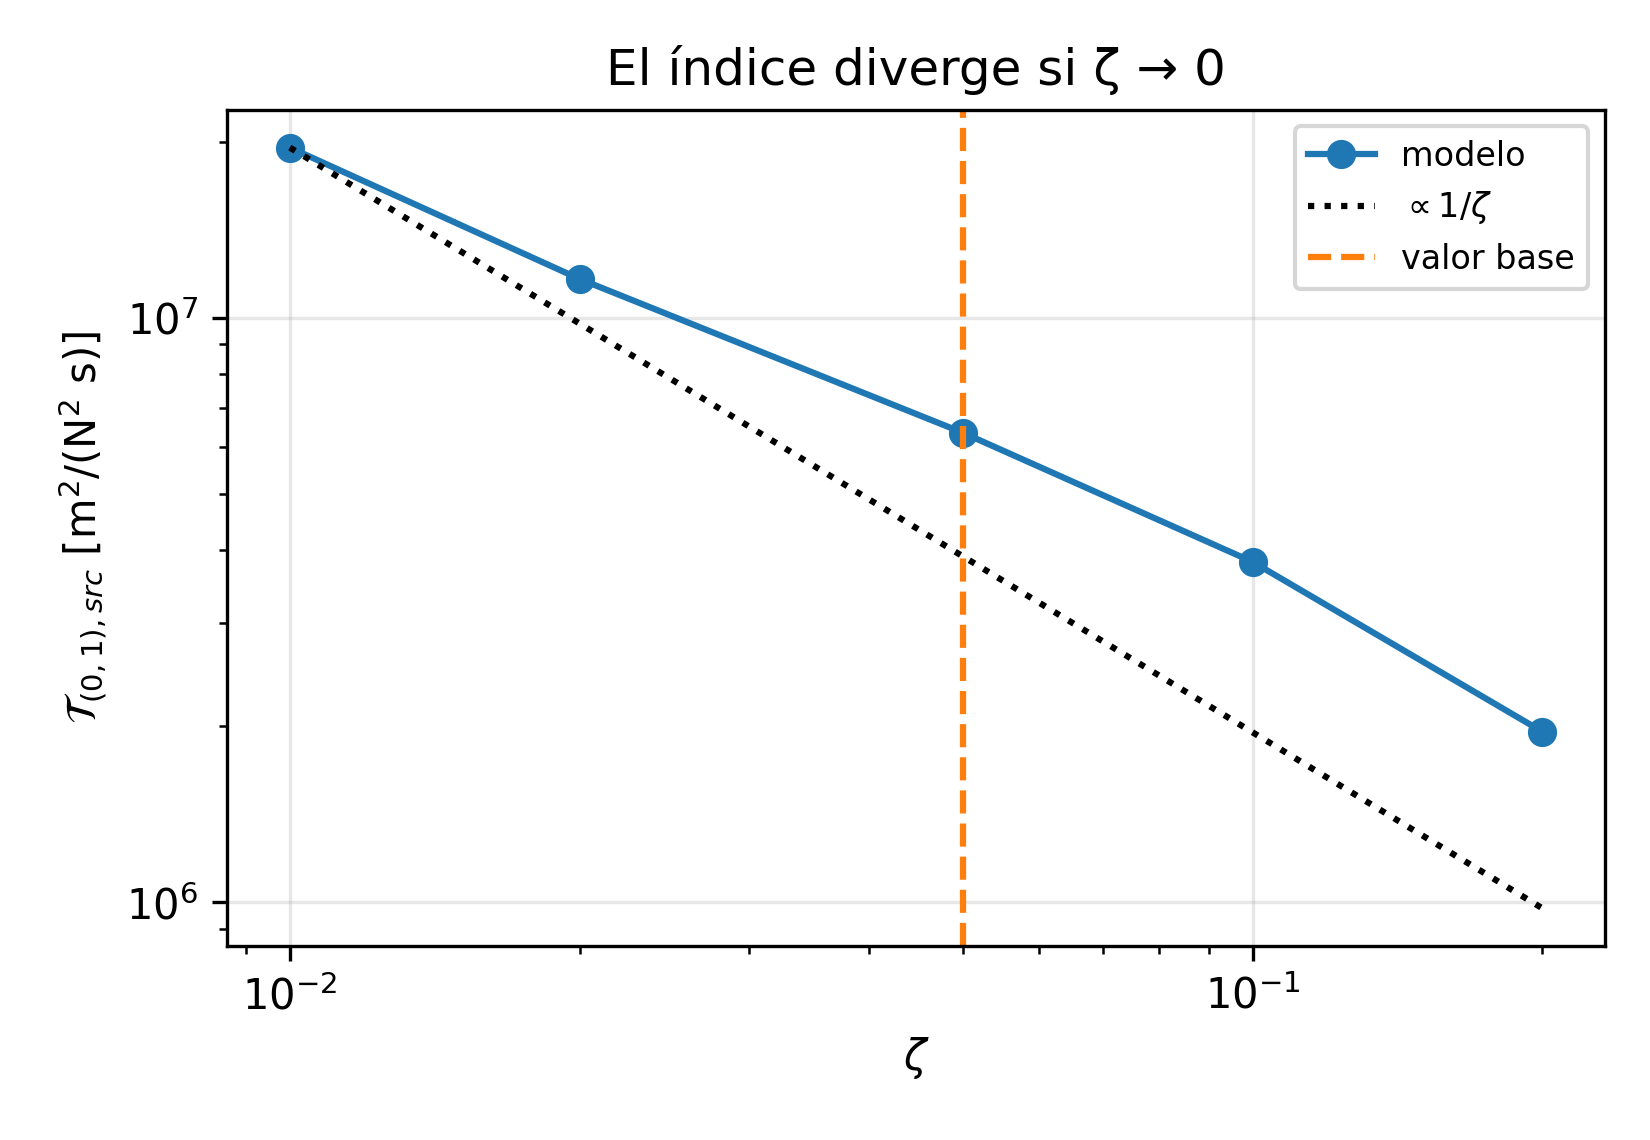
\includegraphics[width=0.55\textwidth]{fig11_sensibilidad_zeta.png}
\caption{Dependencia del índice de transmisión con el amortiguamiento.}
\label{fig:zeta}
\end{figure}

\subsection{Efecto de la araña en el hub}\label{sec:hub}

\begin{table}[H]
\centering\small
\caption{Comparación entre el centro fijo del anteproyecto y el hub libre
con la araña.}
\label{tab:hub}
\begin{tabular}{@{}lcc@{}}
\toprule
 & Centro fijo & Hub libre, $m_a=50$ mg \\
\midrule
Primera frecuencia transversal & 112.8 Hz & 2.50 Hz \\
Modos transversales en 1--1000 Hz & 196 & 197 \\
$\mathcal{T}/\mathcal{T}_{src}$ mismo radial (1--1000 / 5--30 Hz) & $6.6\times10^{-2}$ / $1.5\times10^{-2}$ & $6.9\times10^{-2}$ / $1.3\times10^{-2}$ \\
$\mathcal{T}/\mathcal{T}_{src}$ a $90^\circ$ (1--1000 / 5--30 Hz) & $8.6\times10^{-3}$ / $4.1\times10^{-4}$ & $1.1\times10^{-2}$ / $2.7\times10^{-4}$ \\
$\mathcal{T}/\mathcal{T}_{src}$ radial opuesto (1--1000 / 5--30 Hz) & $9.8\times10^{-3}$ / $1.0\times10^{-5}$ & $1.2\times10^{-2}$ / $1.7\times10^{-4}$ \\
\bottomrule
\end{tabular}
\end{table}

La araña reduce la primera frecuencia transversal en un factor de 45 y
añade un modo de muy baja frecuencia. En la banda de presas, la transmisión
hacia el radial opuesto aumenta en un factor $\approx17$, porque el hub
libre actúa como puente entre radiales. La transmisión por el propio radial
de la presa casi no cambia. Estos resultados justifican adoptar el hub libre
con la araña como modelo principal del ciclo 3.

% =====================================================================
\section{Dificultades y retos pendientes}
% =====================================================================

\begin{itemize}
    \item \textbf{Elección de la métrica de transmisión.} El índice
    integrado en una banda ancha queda dominado por los modos globales y
    pierde la información direccional (tabla~\ref{tab:T}). Se requiere
    comparar geometrías tanto en la banda de presas como con una métrica
    temporal, como la amplitud o el tiempo de primera llegada.
    \item \textbf{Linealidad de la espiral.} La pretensión espiral de
    $9.7\uN$ corresponde a una deformación de $\approx71\,\%$ si se usa el
    módulo inicial de 3 MPa, lo cual está fuera del régimen lineal de la
    seda viscosa. Esto solo afecta a los modos en el plano, porque la
    familia transversal no depende de $\kappa$
    (sección~\ref{sec:ajustes}); para los modos en el plano se debe usar un
    módulo tangente. En los radiales la deformación de pretensión es de
    $0.085\,\%$ y el modelo lineal es adecuado.
    \item \textbf{Masa del pegamento.} No se encontró un valor de masa por
    unidad de longitud de las gotas de la espiral de captura; por ahora
    solo se incluye la fibra. Esa masa adicional reduciría las frecuencias
    y la velocidad de onda.
    \item \textbf{Amortiguamiento.} $\zeta=0.05$ proviene de ensayos de
    histéresis cuasiestáticos; el amortiguamiento a pequeña amplitud y la
    resistencia aerodinámica pueden ser distintos. Por eso las comparaciones
    entre geometrías se harán con índices normalizados y con análisis de
    sensibilidad (figura~\ref{fig:zeta}).
    \item \textbf{Simplificaciones geométricas.} La red es circular,
    simétrica y horizontal (sin peso), y el marco es rígido. Las redes
    reales son verticales y asimétricas, y el peso de la araña redistribuye
    las pretensiones \cite{yavuz2024}.
\end{itemize}

% =====================================================================
\section{Porcentaje de avance}\label{sec:porcentaje}
% =====================================================================

\begin{table}[H]
\centering\small
\caption{Avance por ciclo, ponderado por semanas del cronograma.}
\begin{tabular}{@{}lccc@{}}
\toprule
Ciclo & Peso & Avance del ciclo & Aporte \\
\midrule
Ciclo 1 --- Definición y modelado (sem.\ 1--6) & 33.3\,\% & 100\,\% & 33.3\,\% \\
Ciclo 2 --- Caracterización (sem.\ 7--12) & 33.3\,\% & 100\,\% & 33.3\,\% \\
Ciclo 3 --- Simulación comparativa (sem.\ 13--16) & 22.2\,\% & 0\,\% & 0\,\% \\
Cierre (sem.\ 17--18) & 11.1\,\% & 0\,\% & 0\,\% \\
\midrule
\textbf{Total} & 100\,\% & & \textbf{66.7\,\%} \\
\bottomrule
\end{tabular}
\end{table}

% =====================================================================
\section{Actividades futuras y ajustes al cronograma}
% =====================================================================

\begin{table}[H]
\centering\small
\begin{tabular}{@{}cp{14cm}@{}}
\toprule
Sem. & Actividad (con ajustes) \\
\midrule
13 & Definir configuraciones: barridos de $N$ (dentro de 20--35), de la
separación $\Delta$ de la espiral, del espaciado (lineal o geométrico) y de
$T^S/\bar{T}^R$, respetando siempre \eqref{eq:recurrencia}. Adoptar el hub
libre con la araña como modelo principal. \\
14 & Definir los casos de perturbación: posición radial y angular de la
presa, y dirección transversal o en el plano. Implementar la métrica
temporal de primera llegada junto al índice en la banda de 5--30 Hz. \\
15 & Simular cada configuración y calcular los índices normalizados. \\
16 & Comparar espectros, modos y receptancias entre configuraciones;
analizar la sensibilidad a $\zeta$ y a la masa del pegamento. \\
17--18 & Conclusiones, artículo y sustentación (sin cambios). \\
\bottomrule
\end{tabular}
\end{table}

% =====================================================================
% REFERENCIAS (formato IEEE, numeradas en orden de aparición)
% =====================================================================
\begin{thebibliography}{99}

\bibitem{ewins2000}
D.~J. Ewins, \textit{Modal Testing: Theory, Practice and Application}, 2nd~ed.
Baldock, U.K.: Research Studies Press, 2000.

\bibitem{inman2014}
D.~J. Inman, \textit{Engineering Vibration}, 4th~ed.
Upper Saddle River, NJ, USA: Pearson, 2014.

\bibitem{gosline1999}
J.~M. Gosline, P.~A. Guerette, C.~S. Ortlepp, and K.~N. Savage,
``The mechanical design of spider silks: From fibroin sequence to mechanical
function,'' \textit{J. Exp. Biol.}, vol.~202, no.~23, pp.~3295--3303, 1999,
doi: 10.1242/jeb.202.23.3295.

\bibitem{yavuz2024}
K.~Yavuz, A.~M. Soler, R.~Zaera, and S.~Jahangirov,
``Effect of spider's weight on signal transmittance in vertical orb webs,''
\textit{R. Soc. Open Sci.}, vol.~11, no.~10, Art.~no.~240986, 2024,
doi: 10.1098/rsos.240986.

\bibitem{mortimer2016}
B.~Mortimer, A.~Soler, C.~R. Siviour, R.~Zaera, and F.~Vollrath,
``Tuning the instrument: Sonic properties in the spider's web,''
\textit{J. R. Soc. Interface}, vol.~13, no.~122, Art.~no.~20160341, 2016,
doi: 10.1098/rsif.2016.0341.

\bibitem{adwAraneus}
Animal Diversity Web, ``\textit{Araneus diadematus}: Cross orbweaver,''
Univ. Michigan Museum of Zoology. [Online]. Available:
\url{https://animaldiversity.org/accounts/Araneus_diadematus/}
(accessed Sep.~28, 2026).

\bibitem{stauffer1994}
S.~L. Stauffer, S.~L. Coguill, and R.~V. Lewis,
``Comparison of physical properties of three silks from \textit{Nephila
clavipes} and \textit{Araneus gemmoides},'' \textit{J. Arachnol.}, vol.~22,
no.~1, pp.~5--11, 1994.

\bibitem{landolfa1996}
M.~A. Landolfa and F.~G. Barth,
``Vibrations in the orb web of the spider \textit{Nephila clavipes}: Cues for
discrimination and orientation,'' \textit{J. Comp. Physiol. A}, vol.~179,
pp.~493--508, 1996, doi: 10.1007/BF00192316.

\bibitem{linsobek1998}
L.~H. Lin and W.~Sobek,
``Structural hierarchy in spider webs and spiderweb-type systems,''
\textit{Struct. Eng.}, vol.~76, pp.~59--64, 1998.

\bibitem{wirth1992}
E.~Wirth and F.~G. Barth, ``Forces in the spider orb web,''
\textit{J. Comp. Physiol. A}, vol.~171, pp.~359--371, 1992,
doi: 10.1007/BF00223966.

\bibitem{mortimer2018}
B.~Mortimer, A.~Soler, C.~R. Siviour, and F.~Vollrath,
``Remote monitoring of vibrational information in spider webs,''
\textit{Sci. Nat.}, vol.~105, no.~5--6, Art.~no.~37, 2018.

\end{thebibliography}

\end{document}